\subsection{Mean field theory}

\textbf{From "Many Body Quantum Theory in Condensed Matter Physics" by Henrik Bruus and Karsten Flensberg.}

\begin{tcolorbox}[colback = yellow, title = Physical Context]

The physics of interacting particles is often very complicated because the motion of the individual particles depend on the position of all other, thus these variables become correlated. This is clearly the case for a system of charged particles interacting by Coulomb forces, such as eg. the electron gas. There, the probability to find two electrons in close proximity is expected to be small due to the strong repulsive interaction. Consequently, due to these correlation effects, there is a suppressed density in the neighbourhood of every electron, and there is a correlation hole. 
Nevertheless, in spite of these complications, there are a number of cases where a more crude treatment, not fully including the correlations, gives a good physical model. In these cases, it suffices to include correlations o the average. This means that the effect of the other particles is included as a mean density (or mean field), leaving an effective single particle problem, which is solvable. These mean fields are chosen so that they minimize the free energy, which in turn, ensures that the method is self-consistent. This method is called mean field theory, which allows to neglect detailed dynamics and time-dependent second quantization methods. 

\end{tcolorbox}

\blanky \\

First, consider a system with two types of particles, described by operators ${\bf a}_\nu, {\bf b}_{\mu}$, respectively. In this model, the only interactions present are those between different kind of particles. The Hamiltonian then reads

\begin{equation}
    {\bf H} = {\bf H}_0 + {\bf V}_{\textnormal{int}}, \textnormal{ with } \begin{array}{c}
         {\bf H}_0 = \sum_{\nu} \varepsilon_{\nu}^a {\bf a}_\nu^\dagger {\bf a}_\nu + \sum_{\nu} \varepsilon_{\mu}^b{\bf b}_\mu^\dagger {\bf b}_\mu,  \\
         \\
         {\bf V}_{\textnormal{int}}  = \sum_{\nu\nu', \mu\mu'} {\mathcal V}_{\nu\mu, \nu'\mu'} {\bf a}^\dagger_{\nu} {\bf b}_{\mu}^\dagger {\bf b}_{\mu'} {\bf a}_{\nu'}.
    \end{array}
\end{equation}

Now it may be expected that the density operator ${\bf a}_{\nu}^\dagger {\bf a}_{\nu'}$ and ${\bf b}_{\mu}^\dagger {\bf b}_{\mu'}$, deviate only little from their averages values, $ \langle {\bf a}_{\nu}^\dagger {\bf a}_{\nu'} \rangle$ and  $ \langle {\bf b}_{\nu}^\dagger {\bf b}_{\nu'} \rangle$, respectively. It is natural then to use this deviation as a small parameter and perform an expansion. Let the deviation operators be 

\begin{align}
    {\bf d}_{\nu \nu'} &= {\bf a}_{\nu}^\dagger {\bf a}_{\nu'} - \langle {\bf a}_{\nu}^\dagger {\bf a}_{\nu'} \rangle, & {\bf e}_{\mu \mu'} &= {\bf b}_{\nu}^\dagger {\bf b}_{\nu'} - \langle {\bf b}_{\mu}^\dagger {\bf b}_{\mu'} \rangle.
\end{align}

Then, in terms of these new operators, the Hamiltonian reads

\begin{equation*}
    {\bf H}_{\textnormal{MFT}}  = {\bf H}_0 + {\bf V}_{\textnormal{MFT}} + \cancelto{0}{\sum_{\nu\nu', \mu\mu'} {\bf d}_{\nu \nu'} {\bf e}_{\mu \mu'}}, \textnormal{ where } {\bf V}_{\textnormal{MFT}} = \sum_{\nu\nu', \mu\mu'} {\mathcal V}_{\nu\mu, \nu'\mu'} \left[\begin{array}{c}
         {\bf a}_{\nu}^\dagger {\bf a}_{\nu'} \langle {\bf b}_{\mu}^\dagger {\bf b}_{\mu'} \rangle \\
         \blanky \blanky + {\bf b}_{\mu}^\dagger {\bf b}_{\mu'} \langle {\bf a}_{\nu}^\dagger {\bf a}_{\nu'} \rangle \\
         \blanky \blanky - \langle {\bf a}_{\nu}^\dagger {\bf a}_{\nu'} \rangle \langle {\bf b}_{\mu}^\dagger {\bf b}_{\mu'} \rangle  
    \end{array} \right] + \mathcal{O}(d e).
\end{equation*}

The mean field Hamiltonian $H_{\textnormal{MFT}}$ thus contains only single-particle operators, and thus the original many-body problem has been reduced to a single-particle problem, which can always be solved\footnote{In effect, any quadratic Hamiltonian may be diagonalized since it can be written as ${\bf H} = \sum_{ij} a_i^\dagger {\mathcal{H}}_{ij} a_i^\dagger$. Since this $\bm{ {\mathcal{H}}}$ is hermitian, then there exists a transformation

$$
    {\alpha}_i \rightarrow \sum_{j} U_{ij} a_j, \blanky U \in U(N),
$$

such that $\bm{ {\mathcal{H}}}$ is diagonal: $\sum_{kk'} U_{ik}^\dagger h_{kk'} U_{k'j} = \delta_{ij} \varepsilon_i$. Then, in terms of this new basis, the Hamiltonian then becomes ${\bf H} = \sum_{i} \alpha_i^\dagger \varepsilon_i \alpha_i$, and $\{\varepsilon_i\}$ are thus  $\bm{ {\mathcal{H}}}$'s eigenvalues.}

\blanky \\

Mean field theory may be formulated in a different way: if an interaction term involving the product of two operators, ${\bf A}, {\bf B}$, ie. ${\bf H}_{AB} = {\bf A} {\bf B}$, then the mean field approximation is given by 

$$
    {\bf H}_{AB}^{\textnormal{MFT}} = {\bf A} \langle{\bf B}\rangle + \langle{\bf A} \rangle{{\bf B}} - \langle{\bf A} \rangle\langle{\bf B} \rangle.
$$

The question is then, how to find the averages $\langle {\bf a}_{\nu}^\dagger {\bf a}_{\nu'} \rangle$ and $\langle {\bf b}_{\mu}^\dagger {\bf b}_{\mu'} \rangle$. In principle, there are two possible routes. 

\begin{itemize}
    \item Method 1: these averages are to be determined self-consistently, ie. when calculating the averages 
    
    \begin{align}
        \bar{{\bf n}}_{\nu \nu'}^{a} &= \langle {\bf a}_{\nu}^\dagger {\bf a}_{\nu'} \rangle, & \bar{{\bf n}}_{\mu \mu'}^{b} &= \langle {\bf b}_{\nu}^\dagger {\bf b}_{\nu'} \rangle,
    \end{align}
    
    using the new mean field Hamiltonian, the same answer should be re-obtained. This entails the following prescriptions for $\bar{{\bf n}}_{\nu \nu'}^{a}$ and $\bar{{\bf n}}_{\mu \mu'}^{b}$,
    
     \begin{align} 
     \begin{array}{c}
        \bar{{\bf n}}_{\nu \nu'}^{a} = \langle {\bf a}_{\nu}^\dagger {\bf a}_{\nu'} \rangle_{\textnormal{MFT}} = \frac{1}{\mathcal{Z}_{\textnormal{MFT}}} \Tr \bigg(e^{-\beta {\bf H}_{\textnormal{MFT}}} {\bf a}_{\nu}^\dagger {\bf a}_{\nu'}\bigg) \\ \bar{{\bf n}}_{\nu \nu'}^{b} = \langle {\bf b}_{\mu}^\dagger {\bf b}_{\mu'} \rangle_{\textnormal{MFT}} = \frac{1}{\mathcal{Z}_{\textnormal{MFT}}} \Tr \bigg(e^{-\beta {\bf H}_{\textnormal{MFT}}} {\bf b}_{\mu}^\dagger {\bf b}_{\mu'}\bigg),
     \end{array} \textnormal{ where } \mathcal{Z}_{\textnormal{MFT}} = \Tr \bigg(e^{-\beta {\bf H}_{\textnormal{MFT}}}\bigg).
    \end{align}
    
    Said equations are the self-consistency equations, since the averages are given in terms of the mean field hamiltonian and the mean field partition function, which themselves depend on these averages. \\
    
    \item Method 2: the alternative route consists on using the ${\bf n}_{\nu \nu'}$ which minimizes the free energy $F_{\textnormal{MFT}}$ of the mean field Hamiltonian. Then, 
    
    \begin{equation}
        \begin{split}
            0 &= \frac{d}{d\bar{\bf n}_{\nu \nu'}^{a}} F_{\textnormal{MFT}} = \frac{d}{d\bar{\bf n}_{\nu \nu'}^{a}} \bigg(-\frac{\log \mathcal{Z}_{\textnormal{MFT}}}{\beta}\bigg) = \frac{1}{\mathcal{Z}_{\textnormal{MFT}}} \Tr \bigg(e^{-\beta {\bf H}_{\textnormal{MFT}}} \frac{d}{d\bar{\bf n}_{\nu \nu'}^{a}} {\bf H}_{\textnormal{MFT}} \bigg) \\
            &=\frac{1}{\mathcal{Z}_{\textnormal{MFT}}} \Tr \bigg(e^{-\beta {\bf H}_{\textnormal{MFT}}} \bigg(\sum_{\nu\nu', \mu\mu'} {\mathcal{V}}_{\nu\mu, \nu'\mu'} ({\bf b}_{\mu}^\dagger {\bf b}_\mu - \bar{\bf n}_{\mu\mu'}^{b})\bigg)\bigg) \\
            &= \frac{1}{\mathcal{Z}_{\textnormal{MFT}}} \Tr \bigg(e^{-\beta {\bf H}_{\textnormal{MFT}}} \sum_{\nu\nu', \mu\mu'} {\mathcal{V}}_{\nu\mu, \nu'\mu'} {\bf b}_{\mu}^\dagger {\bf b}_\mu \bigg) - \frac{1}{\mathcal{Z}_{\textnormal{MFT}}} \Tr \bigg(e^{-\beta {\bf H}_{\textnormal{MFT}}} \sum_{\nu\nu', \mu\mu'} {\mathcal{V}}_{\nu\mu, \nu'\mu'}\bar{\bf n}_{\mu\mu'}^{b}\bigg)
            \\
            &= \sum_{\mu \mu'} \frac{1}{\mathcal{Z}_{\textnormal{MFT}}} {\mathcal{V}}_{\nu\mu, \nu'\mu'} \Tr \bigg(e^{-\beta {\bf H}_{\textnormal{MFT}}} {\bf b}_{\mu}^\dagger {\bf b}_\mu \bigg) - \sum_{\mu \mu'} {\mathcal{V}}_{\nu\mu, \nu'\mu'} \bar{\bf n}_{\mu\mu'}^{b} \cancel{\frac{1}{\mathcal{Z}_{\textnormal{MFT}}} \Tr \bigg(e^{-\beta {\bf H}_{\textnormal{MFT}}}}\bigg)\\
            &= \sum_{\mu\mu'} {\mathcal{V}}_{\nu\mu, \nu'\mu'} \bigg(\langle {\bf b}_{\mu}^\dagger {\bf b}_{\mu'} \rangle_{\textnormal{MFT}} - \bar{\bf n}_{\mu\mu'}^{b}\bigg), 
        \end{split}
    \end{equation}
    
    which should hold for any pair $(\nu, \nu')$ and hence, the last parenthesis should vanish. Thus, the self-consistency equation is obtained as well for the second method, making both approaches equivalent. \\
\end{itemize}

Consider the average interaction energy, $\langle {\bf V}_{\textnormal{int}} \rangle$, a natural approximation would be to evaluate the expectation value of the ${\bf a}$ and ${\bf b}$ operators separately, this is 

$$
    \langle {\bf V}_{\textnormal{int}} \rangle \approx \sum_{\nu \nu', \mu \mu'} {\mathcal{V}}_{\nu\mu, \nu'\mu'} \langle {\bf a}_{\nu}^\dagger {\bf a}_{\nu'} \rangle \langle {\bf b}_{\mu}^\dagger {\bf b}_{\mu'} \rangle,
$$

which is equivalent to assuming that the ${\bf a}$ and ${\bf b}$ operators are uncorrelated. This is, in essence, the approximation done in the mean-field approach. In effect, the interaction term can be evaluated using the mean field Hamiltonian 

$$
    \langle {\bf V}_{\textnormal{int}} \rangle_{\textnormal{MFT}} = \frac{1}{\mathcal{Z}_{\textnormal{MFT}}} \Tr \bigg((e^{-\beta {\bf H}_{\textnormal{MFT}}} {\bf V}_{\textnormal{int}}\bigg). 
$$

Since, the mean field Hamiltonian can be separated into a part containing only ${\bf a}$-operators and another term containing only ${\bf b}$-operators, ${\bf H}_{\textnormal{MFT}} = {\bf H}_{\textnormal{MFT}}^a + {\bf H}_{\textnormal{MFT}}^b$, the average factorization yields

\begin{equation}
    \langle {\bf V}_{\textnormal{int}} \rangle_{\textnormal{MFT}} = \sum_{\mu\mu'} {\mathcal{V}}_{\nu\mu, \nu'\mu'} \langle {\bf a}_{\nu}^\dagger {\bf a}_{\nu'} \rangle_{\textnormal{MFT}} \langle {\bf b}_{\mu}^\dagger {\bf b}_{\mu'} \rangle _{\textnormal{MFT}}.
\end{equation}

The mean field theory approach hence provides a consistent a physically sensible method to study interacting system where correlation are less important. Mean field theory is only valid provided $d$ is actually small. This can be checked by calculating $\langle {\bf d} \rangle$, using the neglected term in the Hamiltonian (that concerning the cross term of ${{\bf d}_{\nu \nu'} {\bf e}_{\mu\mu'}}$) as a perturbation, and then compare the result to $\langle {\bf a}_{\nu}^\dagger {\bf a}_{\nu'} \rangle$. If the difference is not negligible, then either the wrong mean field parameter has been chosen or the method simply fails and other more adequate tools must be employed. \\

In practice, it is necessary to assume something about the averages $\langle {\bf a}_{\nu}^\dagger {\bf a}_{\nu'}\rangle$ and $\langle {\bf b}_{\mu}^\dagger {\bf b}_{\mu'} \rangle$. Even though, there is a prescription for which to find which averages are important, there are simply too many combinations. Suppose there are $N$ different quantum numbers, then there are in principle $N^2$ combinations, which then yields $N^2$ coupled non-linear equations, which is only tractable for small systems. Often, symmetry arguments can help in reducing the number of parameters. Suppose for example that the system's Hamiltonian has translational symmetry, such that the momentum space is a natural choice. For a system of particles described by $({\bf c} \blanky {\bf c}^\dagger)$-operators, then 

\begin{equation}
    \langle {\bf c}_{{\bf k}}^\dagger {\bf c}_{{\bf k}'} \rangle = \frac{1}{\mathcal{V}} \int_{\mathds{R}^6} d{\bf x} d{\bf x}' e^{-i {\bf k}' \cdot {\bf x}'} e^{i {\bf k} \cdot {\bf x}} \langle \Psi^\dagger({\bf x}) \Psi({\bf x}') \rangle.
\end{equation}

It is natural to assume that the system is homogenous, which means that 

\begin{equation}
    \langle \Psi^\dagger({\bf x}) \Psi({\bf x}') \rangle = f({\bf x} - {\bf x}') \Rightarrow \langle {\bf c}_{{\bf k}}^\dagger {\bf c}_{{\bf k}'} \rangle = \langle {\bf n}_{\bf k} \rangle \delta_{{\bf k}{\bf k}'}.
\end{equation}

The homogeneity assumption is however not always true, since in some cases the system's symmetry is lower than that of the Hamiltonian. Eg. if the system spontaneously orders into a state with a spatial density variation, like a wave formation, then the average $\langle \Psi^\dagger({\bf x}) \Psi({\bf x}') \rangle$ is not a function of ${\bf x} - {\bf x}'$ only. Instead it has a lower and more restricted symmetry, namely that 

$$
    \langle \Psi^\dagger({\bf x}) \Psi({\bf x}') \rangle = h({\bf x}, {\bf x}') \textnormal{ with } h({\bf x}, {\bf x}') = h({\bf x} + {\bf R}, {\bf x}' + {\bf R}), \textnormal{ ${\bf R}$ a lattice vector}.
$$

\begin{tcolorbox}[colback = yellow, title = Physical Context]

This kind of crystal structure exists in nature and when it happens, the system undergoes a broken symmetry phenomena. It is important to realize that this solution cannot be found by taking the homogeneity assumption but instead by calculating $ \langle {\bf c}_{{\bf k}}^\dagger {\bf c}_{{\bf k} + {\bf Q}} \rangle$, leading to the possibility of this quantity being finite, where ${\bf R} \cdot {\bf Q} = 2\pi$. Thus, the choice of the proper mean field parameters requires physical motivation about which possible states one expects. 

\end{tcolorbox}

\blanky \\

\paragraph{\textgoth{Hartree-Fock theory}}

Mean field theory's methods, upto now, concern only interaction between different particles, wherein correlation terms are replaced by their average values plus small corrections. For interactions between identical particles this, however, does not exhaust the possibilities and only includes the so-called Hartree term, requiring a more general approximation scheme, given by the Hartree-Fock approximation. Consider a quantum system of interacting particles, whose Hamiltonian is given by 
\begin{equation}
    {\bf H} = {\bf H}_0 + {\bf V}_{\textnormal{int}}, \textnormal{ with } \begin{array}{c}
         {\bf H}_0 = \sum_{\nu} \varepsilon_{\nu} {\bf c}_{\nu}^\dagger {\bf c}_{\nu}\\
         \\
         {\bf V}_{\textnormal{int}}  = \frac{1}{2} \sum_{\nu\nu', \mu\mu'} {\mathcal V}_{\nu\mu, \nu'\mu'} {\bf c}_{\nu}^\dagger {\bf c}_{\mu}^\dagger {\bf c}_{\mu'} {\bf c}_{\nu'}.\\
    \end{array}
\end{equation}

The theory's main idea is that the operator $\rho_{\mu \mu'} = {\bf c}_{\mu}^\dagger {\bf c}_{\mu'}$ is large only when the average $\langle \rho_{\mu \mu'} \rangle$ is non-zero. For most $(\nu \nu')$-combinations, the average $\langle \rho_{\nu \nu'} \rangle$ is zero. Therefore, the four-body interaction term may be rewritten in terms of a deviation from the average value

$$
    {\bf c}_{\nu}^\dagger \bigg({\bf c}_{\mu}^\dagger {\bf c}_{\mu'} - \langle {\bf c}_{\mu}^\dagger {\bf c}_{\mu'} \rangle \bigg) {\bf c}_{\nu'} + {\bf c}_{\nu}^\dagger {\bf c}_{\nu'} \langle {\bf c}_{\mu}^\dagger {\bf c}_{\mu'}\rangle.
$$

If $\nu' \neq \mu$, then ${\bf c}_{\nu}$ operator commutes with the parenthesis, which is true upto zero-measure sets. With this assumption, then

\begin{equation}
    \begin{split}
    {\bf c}_{\nu}^\dagger \bigg({\bf c}_{\mu}^\dagger {\bf c}_{\mu'} - \langle {\bf c}_{\mu}^\dagger {\bf c}_{\mu'} \rangle \bigg) {\bf c}_{\nu'} &+ {\bf c}_{\nu}^\dagger {\bf c}_{\nu'} \langle {\bf c}_{\mu}^\dagger {\bf c}_{\mu'}\rangle \overset{{\mu \neq \nu'}}{=} {\bf c}_{\nu}^\dagger {\bf c}_{\nu'} \bigg({\bf c}_{\mu}^\dagger {\bf c}_{\mu'} - \langle {\bf c}_{\mu}^\dagger {\bf c}_{\mu'} \rangle \bigg) + {\bf c}_{\nu}^\dagger {\bf c}_{\nu'} \langle {\bf c}_{\mu}^\dagger {\bf c}_{\mu'}\rangle \\
    &= \bigg({\bf c}_{\nu}^\dagger {\bf c}_{\nu'} - \langle {\bf c}_{\nu}^\dagger {\bf c}_{\nu'} \rangle\bigg) \bigg({\bf c}_{\mu}^\dagger {\bf c}_{\mu'} - \langle {\bf c}_{\mu}^\dagger {\bf c}_{\mu'} \rangle \bigg) + {\bf c}_{\nu}^\dagger {\bf c}_{\nu'} \langle {\bf c}_{\mu}^\dagger {\bf c}_{\mu'}\rangle - {\bf c}_{\mu}^\dagger {\bf c}_{\mu'} \langle {\bf c}_{\nu}^\dagger {\bf c}_{\nu'} \rangle - \langle {\bf c}_{\mu}^\dagger {\bf c}_{\mu'} \rangle \langle {\bf c}_{\nu}^\dagger {\bf c}_{\nu'} \rangle.
    \end{split}
\end{equation}

The first term is proportional to the deviation squared and then may be neglected, yielding the Hartree approximation for interactions

\begin{equation}
\begin{split}
    {\bf V}_{\textnormal{int}}^{\textnormal{HF}} = \frac{1}{2} \sum_{\nu\nu', \mu\mu'} {\mathcal V}_{\nu\mu, \nu'\mu'} \bigg[ \bar{\bf n}_{\mu \mu'} {\bf c}_{\nu}^\dagger {\bf c}_{\nu'} + \bar{\bf n}_{\nu \nu'} {\bf c}_{\mu}^\dagger {\bf c}_{\mu'} - \bar{\bf n}_{\nu \nu'} \bar{\bf n}_{\mu \mu'}\bigg],
\end{split}
\end{equation}

which is the same result that would be obtained if the $(\nu \nu')$ and $(\mu \mu')$-operators were considered to be from different kinds of particles. However, this is not yet the full result, since the $\mu$ and $\nu$-labelled operators represent identical, indistinguishable particles and there is therefore one combination not accounted for by the Hartree approximation, the so-called Fock exchange term. This new term appears since the product of four one-body operators also gives a large contribution if $\langle{\bf c}_{\nu}^\dagger {\bf c}_{\nu'} \rangle$ finite. To derive the mean field contribution from this possibility the $\langle {\bf c}_{\nu}^\dagger {\bf c}_{\mu'} \rangle$ term must first be replaced by its average value and do the same with the combination of $\langle {\bf c}_{\mu}^\dagger {\bf c}_{\nu'} \rangle$, thus yielding 

\begin{equation}
    {\bf V}_{\textnormal{int}}^{\textnormal{Fock}} = - \frac{1}{2} \sum_{\nu\nu', \mu\mu'} {\mathcal V}_{\nu\mu, \nu'\mu'} \bigg[ \bar{\bf n}_{\nu \mu'} {\bf c}_{\mu}^\dagger {\bf c}_{\nu'} + \bar{\bf n}_{\mu \nu'} {\bf c}_{\nu}^\dagger {\bf c}_{\mu'} - \bar{\bf n}_{\mu \nu'} \bar{\bf n}_{\nu \mu'}\bigg].
\end{equation}

Therefore, the final mean field Hamiltonian within the Hartree-Fock approximation is 

\begin{equation}
    {\bf H}^{\textnormal{HF}} = {\bf H}_0 + {\bf V}_{\textnormal{int}}^{\textnormal{Hartree}} + {\bf V}_{\textnormal{int}}^{\textnormal{Fock}}.
\end{equation}

\blanky \\

\paragraph{\textbf{Homogeneous electron gas}}

Consider the example of a translationally invariant homogeneous electron gas, wherein the expectation value $\langle {\bf c}_{\bf k}^\dagger {\bf c}_{\bf k'} \rangle$ is diagonal. From the Hartree-Fock approximation, the Hamiltonian for this system reads 
\begin{align}
    {\bf H}^{\textnormal{HF}} = \sum_{{\bf k} \sigma} \varepsilon_{\bf k}^{\textnormal{HF}} {\bf c}_{{\bf k} \sigma}^\dagger {\bf c}_{{\bf k} \sigma}, \textnormal{ where } \begin{split}
        \varepsilon_{\bf k}^{\textnormal{HF}} &= \varepsilon_{\bf k} + \sum_{{\bf k}' \sigma'} [V(0) - \delta_{\sigma\sigma'} V({\bf k}- {\bf k}')] {\bf n}_{{\bf k}' \sigma'} \\
        &= \varepsilon_{\bf k} + V(0) N - \sum_{{\bf k}' \sigma'} V({\bf k}- {\bf k}') {\bf n}_{{\bf k'} \sigma'}.
    \end{split}
\end{align}

The second term is the interaction with the average electron charge. In condensed matter systems, it is normally cancelled out by an equally large term due to the positively charged ionic background. The third term is precisely the exchange correlation term. \\

The Hartree-Fock approach depends crucially on what averages are assumed to be finite, and these assumptions must be based on physical knowledge or clever guess-work. For example, in the previous example, spin symmetry is assumed to be maintained, which then implies that $\langle {\bf c}_{{\bf k} \downarrow} {\bf c}_{{\bf k}\downarrow} \rangle = \langle {\bf c}_{{\bf k} \uparrow} {\bf c}_{{\bf k}\uparrow} \rangle$. Should this not be the case, a ferromagnetic solution may be obtained. \\

\paragraph{\textbf{Broken Symmetry}}

Mean field theory is often used to study phase transitions and thus changes of symmetry. For a given Hamiltonian with some symmetry (eg. translational symmetry, rotational symmetry in real space or in spin space), there exists an operator which reflects this symmetry and therefore commutes with the Hamiltonian (eg. translation operator, rotation operator in either real or spin space). Since the operator and the Hamiltonian commute, a common set of eigenstates exists. Consider for example, the case of a liquid of particles, wherein the Hamiltonian has translational symmetry. Thus, if ${\mathcal{T}}({\bf R})$ is the translation operator which displaces all particles coordinates by an ${\bf R}$-vector, then $[{\bf H}, {\mathcal{T}}({\bf R})] = 0$. Then, given that this translation operator is in reality a semigroup and given Stone's theorem, then ${\mathcal{T}} = e^{i {\bf R} \cdot {\bf P}}$, where $P$ is the total momentum operator. The total momentum operator is then a conserved quantity, given by 

$$
    {\bf P} = \hbar \sum_{{\bf k} \sigma} {\bf k} {\bf c}^\dagger_{{\bf k} \sigma} {\bf c}_{{\bf k} \sigma}.
$$

An orthonormal basis of states $\ket{{\bf P}}$ with definite total momentum may be chosen. This fact can be used to "prove" the unphysical nature of a density wave. In effect, a ${\bf Q}$-density wave can be written in terms of its Fourier components as 

$$
\rho({\bf Q}) = \sum_{{\bf k}\sigma} {\bf c}_{{\bf k}\sigma}^\dagger {\bf c}_{{\bf k + Q}\sigma}.
$$

Said Forier transform has a finite expectation value. However, it holds as well that

$$
\langle {\bf c}_{{\bf k}\sigma}^\dagger {\bf c}_{{\bf k} + {\bf Q}\sigma} \rangle = \frac{1}{\mathcal{Z}} \sum_{{\bf P}} e^{-\beta E_{{\bf P}}} \bra{{\bf P}} {\bf c}_{{\bf k}\sigma}^\dagger {\bf c}_{{\bf k + Q}\sigma} \ket{{\bf P}} = 0,
$$

since ${\bf c}_{{\bf k}\sigma}^\dagger {\bf c}_{{\bf k + Q}\sigma} \ket{{\bf P}}$ has momentum ${\bf P} - {\bf Q}$ and is thus orthogonal to ${\bf P}$. Then, according to this result, crystals do not exist. In the same way, magnetism, superconductivity and other physical phenomenon do not exist as well. What is wrong? The previous result breaks down if the sum of states in the thermodynamical average is restricted. Even though crystals with different spatial reference points (or ferromagnets with magnetizations in different directions) have formally the same energy, they are effectively decoupled due to the large energy barrier it takes to melt and then recrystallize into a new state with a shifted distance (or direction of magnetization). In those cases, where many states of the system are degenerate but separated by large energy barriers, it does not make sense to include them on equal footing in the statistical average, since they correspond to macroscopically totally different configurations. Therefore, the ergodicity postulate does not hold, giving rise to a phase space of physically separated sections, which is often illustrated by the double barrier model of phase transitions. 

When at some critical temperature, the thermodynamical state of the system develops a non-zero expectation value of some macroscopic quantity, which has less symmetries than the original Hamiltonian, it is called spontaneous symmetry breaking. The quantity which signals that a phase transition has occurred is the order parameter. Some examples of order parameters are presented in \cref{order paras table}.

\begin{table}[!h]
\centering
\begin{tabular}{ |p{5cm}||p{5cm}|p{4cm}|  }
 \hline
 \multicolumn{3}{|c|}{Examples of Spontaneous Symmetry Breaking} \\
 \hline
 \textbf{Phenomena} & \textbf{Order parameter} & \textbf{ Order parameter} \\
 & \textbf{ physical } & \textbf{ mathematical }\\
 \hline
 crystal & density wave & $\sum_{{\bf k}} \langle {\bf c}_{{\bf k}}^\dagger {\bf c}_{{\bf k} + {\bf Q}} \rangle $\\
 ferromagnet & magnetization & $\sum_{{\bf k}} \langle {\bf c}_{{\bf k}\uparrow}^\dagger {\bf c}_{{\bf k}\uparrow} - {\bf c}_{{\bf k}\downarrow}^\dagger {\bf c}_{{\bf k}\downarrow} \rangle$\\
 Bose-Einstein condensate & population of ${\bf k}=0$-state & $\langle {\bf a}_{{\bf k} = 0}^\dagger \rangle$\\
 superconductor & pair condensate & $\langle {\bf c}_{{\bf k} \uparrow}^\dagger {\bf c}_{-{\bf k}\downarrow} \rangle$ \\
 \hline
\end{tabular}
 \caption{Typical examples of spontaneous symmetry breakings and their correspondent order parameters. }
 \label{order paras table}
\end{table}

In order to avoid the paradox obtained before with the wave density, the possibility of phase transitions must be explicitly included into the theory. In the mean field approach, the trick is to include the order parameter in the choice of finite mean fields, and, of course, show that the resulting mean field Hamiltonian leads to a self-consistent finite result. \\

\paragraph{\textbf{Ferromagnetism: The Heisenberg model}}

In ionic magnetic crystals, the interaction between the magnetic ions is due to the exchange interactions originating from the Coulomb interactions. The theory's effective Hamiltonian is given by 

\begin{equation}
    {\bf H} = - 2 \sum_{i \sim j} J_{ij} {\spin}_i \cdot \spin, \textnormal{ where } i \sim j \textnormal{ if } ||i-j||_1 = 1.
\end{equation}

The interaction, which depends only on the inter-ion distance, is generally short ranged and assumed to be simply $J_{ij} = J_0 \delta_{||i-j||_1, 1}$, ie. is only non-zero for nearest-neighbours. \\

If $J<0$, the spins tend to become anti-parallel whereas for $J>0$, it is energetically favourable for the spins to be parallel, the first case corresponds to the antiferromagnetic case while the latter to the ferromagnetic case. For now, consider only the ferromagnetic case, $J > 0$. \\

As the model stands, it is inherently complicated and cannot be solved in general, the spins of the individual ions being strongly correlated. However, a mean field solution can be readily be found to give sensical physical results. The mean field decomposition reads

\begin{equation}
    {\bf H} \approx {\bf H}_{\textnormal{MF}} = -2 \sum_{i \sim j} J_{ij} \bigg( \langle \spin_i \rangle \spin_j + \spin_i\langle \spin_j \rangle - \langle \spin_i \rangle \langle \spin_j \rangle \bigg).
\end{equation}

From symmetry arguments it is expected that the expectation value of $\langle {\bf S}_i \rangle$ is zero, since all directions are equivalent. But this is not the right answer, since a symmetry has been broken, and has to be presumed to be non-zero. Furthermore, since the system has translational symmetry, this average is expected to be position coordinate independent. This would not be the case for an antiferromagnetic solution, wherein position is important since the spins point on opposite directions on even and odd sites. In the ferromagnetic case, a finite but spatially independent average spin polarization is studied. In particular, if the $z$-axis is chosen to lie along the direction of the magnetization, then the mean field assumption is

$$
    \langle \spin_i \rangle = \langle \spin_z \rangle {\bf e}_z,
$$

and each spin's magnetic moment ${\bf m}$, which by assumption is equal for all sites, reads

$$
    {\bf m} = 2 \sum_{j} J_{ij} \langle \spin_z \rangle {\bf e}_z = 2n J_0 \langle \spin_z \rangle {\bf e}_z, \textnormal{ where $n$ is the number of neighbours}. 
$$

For a square lattice, $\Lambda \subseteq \mathds{Z}^d$ and $n = 2d$. Then men field Hamiltonian is then

$$
    {\bf H}_{\textnormal{MFT}} = - 2 \sum_{i} {\bf m} \cdot \spin_i + m N \langle \spin_z \rangle,
$$

which is now diagonal in the site index and hence easily solved. If the ions are spin-$\frac{1}{2}$ particles, with this simplification, the mean field partition function is 

$$
    {\mathcal{Z}_{\textnormal{MFT}}} = \bigg( e^{\beta m} + e^{-\beta m} \bigg)^N e^{\beta N m \langle \spin_z \rangle} = \bigg[ \bigg( e^{\beta m} + e^{-\beta m} \bigg) e^{\frac{\beta m^2}{2n J_0}} \bigg]^N,
$$

with one term for each possible spin projection. \\

The self-consistency equation is found by minimizing the free energy 

$$
    \frac{\partial F_{\textnormal{MFT}}}{\partial m} = - \frac{1}{\beta} \frac{\partial \log  {\mathcal{Z}_{\textnormal{MFT}}}}{\partial m} = -N \bigg(\frac{e^{\beta m} - e^{-\beta m}}{e^{\beta m} + e^{-\beta m}}\bigg) + N \frac{m}{n J_0} = 0 \Rightarrow \alpha = \tanh(b \alpha), \textnormal{ where } \begin{array}{c}
        \alpha = \frac{m}{nJ_0}  \\
        \\
        b = nJ_0 \beta.  
    \end{array}
$$

For small $\alpha$, the previous equation reads

$$
\alpha \approx b \alpha - \frac{(b\alpha)^3}{3},
$$

from which it is evident that there is no solution for $b < 1$. Thus, the critical temperature $T_c$ can be found since at this temperature magnetism disappears. From the $(b_c = 1)$-condition, it is found that $k_B T_c = n J_0$. Furthermore, for small $\alpha$, the solution for the magnetization can be found 

\begin{align}
    \alpha \approx \frac{1}{b} \sqrt{\frac{3(b-1)}{b}} \Rightarrow m \approx nJ_0 \sqrt{3 \frac{T_c - T}{T_c}}, \textnormal{ valid for } T \rightarrow T_c.    
\end{align}


At $T=0$, where $t \rightarrow\infty$, the solution is $\alpha = 1$ and hence $m = n J_0$. For the functional form of the magnetization in the entire range of temperature, the transcendental equation must be solved numerically. \\

\paragraph{\textbf{The Stoner-Hubbard of metallic ferromagnets}}

In magnets where the electrons both generate magnetic moments and also form conduction bands, the Heisenberg model proves to be inadequate given that the spins are not localized. Metallic magnetism occurs eg. in transition metals, where the conduction bands are formed by the narrower $d$ or $f$ orbitals. The interaction between two particles in those orbitals is stronger than between electrons occupying the more spread out $s$ or $p$ orbitals and hence give a larger correlation between electrons. Typical metals where correlations between conduction band electrons are important for Fe and Ni. \\

Since the short-range of the interaction is important, the physical model -the so-called Hubbard model- must incorporate a simple physical fact. Namely, that the Coulomb interaction between electrons is taken to be point-like in real space, and hence constant in momentum space

\begin{equation}
    {\bf H}_{\textnormal{Hub}} = \sum_{{\bf k} \sigma} \varepsilon_{{\bf k}} {\bf c}_{{\bf k}\sigma}^\dagger {\bf c}_{{\bf k}\sigma} + \frac{U}{2\mathcal{V}} \sum_{\substack{{\bf k}, {\bf k}', {\bf q} \\
          {\sigma \sigma'}}} {\bf c}_{{\bf k+q} \sigma}^\dagger {\bf c}_{{\bf k'-q} \sigma'}^\dagger {\bf c}_{{\bf k}' \sigma'} {\bf c}_{{\bf k}\sigma}.
\end{equation}

Then, the Hartree-Fock approximation scheme may be employed on this model, by searching for a ferromagnetic solution which allows expectation values to depend on the direction of the spin. The mean field parameters are 

\begin{align}
    \langle {\bf c}_{{\bf k}\uparrow}^\dagger {\bf c}_{{\bf k}'\uparrow} \rangle &= \delta_{{\bf k} {\bf k}'} \bar{n}_{{\bf k} \uparrow} & \langle {\bf c}_{{\bf k}\downarrow}^\dagger {\bf c}_{{\bf k}'\downarrow} \rangle &= \delta_{{\bf k} {\bf k}'} \bar{n}_{{\bf k} \downarrow}, 
\end{align}

and the mean-field interaction Hamiltonian becomes 

\begin{align*}
    {\bf V}_{\textnormal{int}}^{\textnormal{MFT}} &= \frac{U}{\mathcal{V}} \sum_{\substack{{\bf k}, {\bf k}', {\bf q} \\
          {\sigma \sigma'}}} \bigg[ {\bf c}_{{\bf k + q}\sigma}^\dagger \langle {\bf c}_{{\bf k'-q}\sigma'}^\dagger {\bf c}_{{\bf k}'\sigma'} \rangle {\bf c}_{{\bf k}\sigma} - \langle {\bf c}_{{\bf k + q}\sigma}^\dagger {\bf c}_{{\bf k}'\sigma'} \rangle {\bf c}_{{\bf k'-q}\sigma'}^\dagger {\bf c}_{{\bf k}\sigma}  \\
          &  \blanky \blanky \blanky \blanky \blanky \blanky \blanky \blanky \blanky \blanky \blanky \blanky \blanky \blanky \blanky \blanky \blanky \blanky   -\frac{1}{2} \bigg( \langle {\bf c}_{{\bf k + q}\sigma}^\dagger {\bf c}_{{\bf k}\sigma} \rangle \langle {\bf c}_{{\bf k' - q}\sigma'}^\dagger {\bf c}_{{\bf k}'\sigma'} \rangle - \langle {\bf c}_{{\bf k + q}\sigma}^\dagger {\bf c}_{{\bf k}'\sigma'} \rangle \langle {\bf c}_{{\bf k' - q}\sigma'}^\dagger {\bf c}_{{\bf k}\sigma} \rangle  \bigg)  \bigg] \\
          &= \frac{U}{\mathcal{V}} \sum_{\substack{{\bf k}, {\bf k}', {\bf q} \\
          {\sigma \sigma'}}} 
          \bigg[ {\bf c}_{{\bf k + q}\sigma}^\dagger {\bf c}_{{\bf k}\sigma} \delta_{{\bf k'-q} \blanky {\bf k}'} \bar{n}_{{\bf k'} \sigma'} - {\bf c}_{{\bf k'-q}\sigma'}^\dagger {\bf c}_{{\bf k}\sigma} \delta_{{\bf k+q} \blanky {\bf k}'} \delta_{\sigma \sigma'} \bar{n}_{{\bf k}' \sigma'} \\
          & \blanky \blanky \blanky \blanky \blanky \blanky \blanky \blanky \blanky \blanky \blanky \blanky \blanky \blanky \blanky \blanky \blanky \blanky  - \frac{1}{2} \bigg(\delta_{{\bf k+q} \blanky {\bf k}} \bar{n}_{{\bf k} \sigma} \delta_{{\bf k'-q} \blanky {\bf k}'} \bar{n}_{{\bf k}' \sigma'} - \delta_{{\bf k+q} \blanky {\bf k}'} \delta_{\sigma \sigma'} \bar{n}_{{\bf k}' \sigma'} \delta_{{\bf k'-q} \blanky {\bf k}} \delta_{\sigma \sigma'} \bar{n}_{{\bf k} \sigma} \bigg) \bigg] \\
          &= U \sum_{\substack{{\bf k}, {\bf k}'\\
          {\sigma \sigma'}}} \bigg[ {\bf c}_{{\bf k}\sigma}^\dagger {\bf c}_{{\bf k}\sigma} \frac{\bar{n}_{{\bf k'} \sigma'}}{\mathcal{V}} - {\bf c}_{{\bf k}\sigma}^\dagger {\bf c}_{{\bf k}\sigma} \delta_{\sigma \sigma'} \frac{\bar{n}_{{\bf k'} \sigma'}}{\mathcal{V}} - \frac{1}{2} \bigg(\bar{n}_{{\bf k} \sigma} \frac{\bar{n}_{{\bf k'} \sigma'}}{\mathcal{V}} - \delta_{\sigma \sigma'} \bar{n}_{{\bf k'} \sigma'} \frac{\bar{n}_{{\bf k} \sigma}}{\mathcal{V}} \bigg)\bigg] \\
          &= U \sum_{{\bf k} \sigma \sigma'} \bigg[{\bf c}_{{\bf k}\sigma}^\dagger {\bf c}_{{\bf k}\sigma} (\bar{n}_{\sigma'} - \delta_{\sigma \sigma'} \bar{n}_{\sigma}) - \mathcal{V} \bar{n}_{\sigma} \bar{n}_{\sigma'} + \mathcal{V} \bar{n}_{\sigma}^2   \bigg], \textnormal{ where } \bar{n}_{\sigma} = \frac{1}{\mathcal{V}} \sum_{{\bf k'}} \langle {\bf c}_{{\bf k'}\sigma}^\dagger {\bf c}_{{\bf k'}\sigma} \rangle \textnormal{ is the spin density}.
\end{align*}

The full Hamiltonian reads

\begin{equation}
    {\bf H}_{\textnormal{MFT}} = \sum_{{\bf k} \sigma} \varepsilon_{{\bf k} \sigma}^{\textnormal{MFT}} {\bf c}_{{\bf k}\sigma}^\dagger {\bf c}_{{\bf k}} - \frac{U \mathcal{V}}{2} \sum_{\sigma \sigma'} \bigg( \bar{n}_{\sigma} \bar{n}_{\sigma'} - \bar{n}_{\sigma}^2 \delta_{\sigma \sigma'} \bigg), \textnormal{ with } \varepsilon_{{\bf k} \sigma}^{\textnormal{MFT}} = \varepsilon_{{\bf k}} + U(n_\uparrow + {\bar n}_\downarrow - \bar{n}_\sigma) = \varepsilon_{\bf k} + U\bar{n}_{\bar{\sigma}}.
\end{equation}

The mean field solution is found via minimization, 

\begin{align*}
    0 &= \frac{d}{d \bar{n}_{\sigma}} F_{\textnormal{MFT}} = \frac{d}{d \bar{n}_{\sigma}} \bigg( - \frac{\log \mathcal{Z}_{\textnormal{MFT}}}{\beta} \bigg) = \frac{1}{\mathcal{Z}_{\textnormal{MFT}}} \Tr \bigg(e^{-\beta {\bf H}_{\textnormal{MFT}}} \frac{d}{d\bar{n}_{\sigma}} {\bf H}_{\textnormal{MFT}} \bigg) \\
    &= - \frac{1}{\mathcal{Z}_{\textnormal{MFT}}} \Tr \bigg[e^{-\beta {\bf H}_{\textnormal{MFT}}} \bigg(\sum_{{\bf k}\sigma} \frac{d \varepsilon_{{\bf k} \sigma}^{\textnormal{MFT}}}{d \bar{n}_{\sigma}} {\bf c}_{{\bf k}\sigma}^\dagger {\bf c}_{{\bf k}\sigma} - \frac{U  \mathcal{V}}{2} \sum_{\sigma \sigma'} ({\bar n}_{\sigma'} + \bar{n}_{\sigma} \delta_{\sigma \sigma'} -2 \bar{n}_{\sigma'} \delta_{\sigma \sigma'} ) \bigg) \bigg] \\
    &= - \frac{1}{\mathcal{Z}_{\textnormal{MFT}}} \Tr \bigg[e^{\beta {\bf H}_{\textnormal{MFT}}} \bigg(\sum_{{\bf k}\sigma} -U {\bf c}_{{\bf k}\sigma}^\dagger {\bf c}_{{\bf k}\sigma}  - \frac{U  \mathcal{V}}{2} \sum_{\sigma \sigma'} ({\bar n}_{\sigma'} - \bar{n}_{\sigma'} \delta_{\sigma \sigma'} ) \bigg) \bigg] \\
    &= U \sum_{{\bf k} \sigma} \langle {\bf c}_{{\bf k}\sigma}^\dagger {\bf c}_{{\bf k}\sigma} \rangle_{\textnormal{MFT}} - \frac{U  \mathcal{V}}{2} \sum_{\sigma \sigma'} ({\bar n}_{\sigma'} - \bar{n}_{\sigma'} \delta_{\sigma \sigma'} ) =  U \langle {\bf c}_{{\bf k}\sigma}^\dagger {\bf c}_{{\bf k}} \rangle_{\textnormal{MFT}} + U \mathcal{V} \bar{n}_{\sigma} \\
    &= \frac{U}{\mathcal{Z}_{\textnormal{MFT}}} \sum_{{\bf k} \sigma} \Tr \bigg[e^{-\beta {\bf H}_{\textnormal{MFT}}} {\bf c}_{{\bf k}\sigma}^\dagger {\bf c}_{{\bf k}\sigma} \bigg] + \frac{U  \mathcal{V}}{2} \sum_{\sigma \sigma'} ({\bar n}_{\sigma'} - \bar{n}_{\sigma'} \delta_{\sigma \sigma'}) \cancel{\frac{1}{\mathcal{Z}_{\textnormal{MFT}}} \Tr \bigg[e^{-\beta {\bf H}_{\textnormal{MFT}}} \mathds{1} \bigg]} \\
    &= \frac{U}{\mathcal{V}} \sum_{{\bf k}} \langle {\bf c}_{{\bf k}\sigma}^\dagger {\bf c}_{{\bf k}\sigma} \rangle_{\textnormal{MFT}} - \frac{U \mathcal{V}}{2} \bigg( 2 \sum_{\sigma'} {\bar n}_{\sigma'} - \sum_{\sigma} {\bar n}_{\sigma} \bigg) \bigg] =  \sum_{\sigma} \bigg[ \sum_{{\bf k}} \frac{U}{\mathcal{V}} \langle {\bf c}_{{\bf k}\sigma}^\dagger {\bf c}_{{\bf k}\sigma} \rangle_{\textnormal{MFT}} + \frac{U \mathcal{V}}{2} {\bar{ n}_{\sigma}} \bigg]\\
    \Rightarrow \bar{n}_{\sigma} &= \frac{1}{\mathcal{V}} \sum_{{\bf k}} \langle {\bf c}_{{\bf k}\sigma}^\dagger {\bf c}_{{\bf k}\sigma} \rangle_{\textnormal{MFT}} = \frac{1}{\mathcal{V}} \sum_{{\bf k}} n_F(\varepsilon_{{\bf k} \sigma}^{\textnormal{MFT}}).
\end{align*}

% revisar esta cuenta porque me quedó con un dos de más

At zero temperature, 

\begin{align}
\begin{array}{c}
    {\bar n}_\uparrow = \int_{\mathds{R}^3} \frac{d {\bf k}}{(2\pi)^3} \blanky \Theta\bigg( \mu - \frac{\hbar^2 k^2}{2m} - U \bar{n}_\downarrow\bigg) = \frac{k_{F\uparrow}^3}{6\pi^2} \\
    {\bar n}_\downarrow = \int_{\mathds{R}^3} \frac{d {\bf k}}{(2\pi)^3} \blanky \Theta\bigg( \mu - \frac{\hbar^2 k^2}{2m} - U \bar{n}_\uparrow\bigg) = \frac{k_{F\downarrow}^3}{6\pi^2},
\end{array}
\textnormal{ where } \frac{\hbar^2 k_{F \sigma}}{2m} + U \bar{n}_{(\sigma)^{*}} = \mu.
\end{align}

Thus, yielding two equations 

\begin{align}
    \frac{\hbar^2}{2m} (6\pi)^{\frac{2}{3}} {\bar n}_{\uparrow}^{\frac{2}{3}} + U {\bar n}_{\downarrow} &= \mu,s & \frac{\hbar^2}{2m} (6\pi)^{\frac{2}{3}} {\bar n}_{\downarrow}^{\frac{2}{3}} + U {\bar n}_{\uparrow} &= \mu.
\end{align}

Let, 

\begin{align*}
    \zeta &= \frac{{\bar n}_{\uparrow}-{\bar n}_{\downarrow}}{{\bar n}}, & \gamma &= \frac{2m U n^{\frac{1}{3}}}{(3\pi^2)^{\frac{3}{2}} \hbar^2}, & {\bar n} &= {\bar n}_{\uparrow} + {\bar n}_{\downarrow},
\end{align*}

then, by subtracting the two equations,

\begin{align}
    {\bar n}_{\uparrow}^{\frac{2}{3}} - {\bar n}_{\downarrow}^{\frac{2}{3}} = \frac{2mU}{\hbar^2} (6\pi)^{-\frac{2}{3}} ({\bar n}_{\uparrow}-{\bar n}_{\downarrow}) \Rightarrow \gamma \zeta = (1+\zeta)^{\frac{2}{3}} - (1-\zeta)^{\frac{2}{3}},
\end{align}

which has three types of solutions:

\begin{itemize}
    \item $\gamma < \frac{4}{3}$: isotropic solution: $\zeta = 0$, which corresponds to a normal state.
    \item $\frac{4}{3} < \gamma < 2^{\frac{2}{3}}$: Partial polarization $0 < \zeta < 1$, which corresponds to a weak ferromagnet.
    \item $\gamma > 2^{\frac{2}{3}}$: Full polarization $\zeta = 1$, which corresponds to a strong ferromagnet. \\
\end{itemize}

The possibility for a magnetic solution can be traced back to the spin dependent eigenenergies, where it is clear that the mean field energy of a given spin direction depends on the occupation of the opposite spin direction, whereas the energy does not depend on the occupation of the same spin direction. This is a consequence of two things: the short range interaction and the exchange term. Both can be understood from the Pauli principle, which ensures that electrons with the same spin never occupy the same spatial orbitals and therefore, if the interaction is short-range, they cannot interact. This leaves interactions between opposite spins as the only possibility. Thus, the interaction energy is lowered by having a polarized ground state, which on the other hand for a fixed density costs kinetic energy. The competition between the kinetic and potential energy gives rise to the phase transition. \\

The Stoner-Hubbard model gives a reasonable account for metallic magnets and is capable of qualitatively explaining the properties of excitations in the spin polarized states. \\

%incluir el grafiquito de transiciones de fase del modelo, sacado del Many Body Quantum Theory yada yada yada de Bruus-Flensberg. 

\paragraph{\textbf{Superconductivity: BCS theory}}

One of the most striking examples of symmetry breaking is the superconducting phase transition. Below the critical temperature the metal which turns superconducting, has no resistance whatsoever, and it exhibits perfect diamagnetism, called Meisner effect, which means that magnetic fields are totally expelled from the interior of the material. These astonishing phenomena result from the superconducting state having a new form of symmetry breaking, namely loss of global gauge invariance. Both the new type of phase and the appearance of an excitation gap are explained by the Bardeen-Cooper-Schrieffer theory. \\

\underline{Breaking of global gauge symmetry and its consequences}. What kind of broken symmetry may give rise to a superconducting state? the relevant symmetry is the global gauge symmetry, ie. all electrons may be added the same constant extra phase without altering the Hamiltonian. The ferromagnetic analog is that all spins can be rotated by some angle without changing the Hamiltonian, due to a global $SO(3)$-symmetry. In that case, a broken $SO(3)$-symmetry, entails that the expectation value $\langle {
\bf S}\rangle$ is not invariant under rotation, since it will change the magnetization's direction. In the same venue, a phase rotation changes the superconducting order parameter, which is of the form $\langle {\bf c}_{\mu} {\bf c}_{\mu'} \rangle$ ie. the expectation value of two annihilation operators. Of course, the number of particles is conserved, but this is not a problem in our setting for we are only interested in superconductors connected to electron reservoirs. 

While it is clear why the finite expectation value $\langle {\bf S} \rangle$ gives a magnetization in the case of a ferromagnet, it is not so clear why broken symmetry in the superconducting case leads to a system without resistance. Moreover, even though the superconducting phase is sensitive to a change in global phase, it is clear that a constant phase cannot have any measurable effect, since all expectation values are given in terms of the absolute square of the wave function. However, phase gradients can have an effect. \\

Consider a superconducting state, which is ascribed by a phase which depends on the position, $\phi({\bf x})$, and varies extremely slowly, such that it takes a macroscopic distance to see any significant changes in $\phi({\bf x})$. For any other non-superconducting system, it would not make sense to talk about a quantum mechanical phase difference over macroscopic distances, simply because quantum coherence is destroyed by all sorts of scattering events on rather short lengths ($\sim 10 nm$ for metals). To argue that the superconducting state depends on phase differences over macroscopic distances is unusual and implies that superconductivity is a macroscopic quantum phenomenon. \\

Consider the following unitary transformation, which changes the phase 

$$
    U = \exp \bigg( i \int_{\mathds{R}^3} d{\bf x} \blanky \rho({\bf x}) \phi({\bf x}) \bigg), \textnormal{ where } \rho({\bf x}) =  \Psi^{\dagger}({\bf x}) \Psi({\bf x}).
$$

When applied to quantum field operators it has the following properties 

\begin{align}
    {\tilde \Psi}({\bf x}) &= U {\Psi}({\bf x}) U^{-1} = \exp\bigg(i \int_{\mathds{R}^3} d{\bf x} \blanky \rho({\bf x}) \phi({\bf x}) \bigg) {\Psi}({\bf x}) \exp\bigg(-i \int_{\mathds{R}^3} d{\bf x} \blanky \rho({\bf x}) \phi({\bf x}) \bigg) \\
    &= {\Psi}({\bf x}) e^{-i \phi({\bf x})} \\
    {\tilde \Psi}^\dagger({\bf x}) &= U {\Psi}^\dagger({\bf x}) U^{-1} = {\Psi}^\dagger({\bf x}) e^{i \phi({\bf x})}.
\end{align}

These equations follow from the differential equation problem

$$
    \left\{\begin{array}{cc}
         \frac{\delta \tilde{\Psi}({\bf x})}{\delta \phi({\bf x'})} = i U [\rho({\bf x}'), \Psi({\bf x})] U^{-1} = i \tilde{\Psi}({\bf x}) \delta({\bf x}-{\bf x}')  \\
         \tilde{\Psi}({\bf x})\bigg|_{\phi = 0} = \Psi({\bf x})
    \end{array} \right.
$$

The transformed partition function is given by 

$$
    \tilde{\mathcal{Z}} = \Tr' [U e^{-\beta {\bf H}} U^{-1}] = \Tr' [e^{-\beta \tilde{\bf H}}],
$$

note that, if the cyclic property of the trace had been used, $U$ would have disappeared all-together. However, when dealing with systems with broken symmetry, the sum-over-states has to be restricted so that the the cyclic property does not hold. In other words, the trace is restricted due to the spontaneous symmetry breaking. The transformation only changes the kinetic term of the Hamiltonian, since the Coulomb interaction term, the impurity scattering term and the phonon coupling term only involves the, phase-invariant, electron density operator $\rho({\bf x})$. The kinetic term reads

\begin{equation}
    \begin{split}
        \tilde{\bf H} &= \frac{1}{2m_e} \int_{\mathds{R}^3} d{\bf x} \blanky {\bf \Psi}^\dagger({\bf x}) e^{i\phi({\bf x)}} \bigg(\frac{\hbar}{i} \nabla + e {\bf A}\bigg)^2 e^{-i\phi({\bf x)}} {\bf \Psi}({\bf x}) \\
        &= \frac{1}{2m_e} \int_{\mathds{R}^3} d{\bf x} \blanky {\bf \Psi}^\dagger({\bf x}) \bigg(\frac{\hbar}{i} \nabla + e {\bf A} - \hbar \nabla \phi({\bf x})\bigg)^2 {\bf \Psi}({\bf x}) \\
        &= {\bf H} - \hbar \int_{\mathds{R}^3} d{\bf x} \blanky \nabla \phi({\bf x}) \cdot {\bf J}({\bf x}) - \frac{\hbar}{2m_e} \rho({\bf x}) (\nabla \phi({\bf x}))^2.
    \end{split}
\end{equation}

Therefore, the phase is a macroscopic quantity. The lowest free energy condition can be found by minimizing the free energy with respect to the phase. It is clear that the energy does not depend with $\phi$ itself, but on its gradient, hence

\begin{equation}
\begin{split}
    \frac{\delta F}{\delta \phi({\bf x})} &= - \hbar \int_{\mathds{R}^3} d{\bf x} \blanky {\bf J}({\bf x}) - \frac{\hbar}{m_e} \rho({\bf x}) \nabla \phi({\bf x}) \\
    &= - \langle {\bf J}({\bf x}) \rangle + \frac{\hbar}{m_e} \langle \rho({\bf x}) \rangle \nabla \phi({\bf x}) = 0   \Rightarrow \langle {\bf J} \rangle = \frac{\hbar \rho_0}{m_e} \nabla \phi.
\end{split}
\end{equation}

\begin{tcolorbox}[colback = yellow, title = Physical Context]

The previous equation's physical meaning is that, by forcing a phase gradient onto the system, it minimizes its energy by carrying a current even in thermodynamical equilibrium, giving rise to a non-equilibrium current. In reality, the electron density should only include those electrons participating in the superconducting condensate, the so-called superfluid. In this derivation, it is assumed all electrons participate. \\

In the normal state of metals, a current is always associated with a non-equilibrium state, where energy is constantly dissipated from the driving source and absorbed in the conductor. Of course, there is an energy cost for the system to carry the current, but as long as this cost is smaller than the alternative which is to go out of the superconducting state, the current carrying state is chosen. The critical current is reaches when the energies are equal, and then the superconductor goes into the normal state. Thus, when a phase gradient is imposed to a system, wherein the energy is assumed to depend on phase differences on a macroscopic scale, it unavoidably leads to the conclusion that the system will carry a dissipationless current in order to minimize the energy cost of the phase gradient. Finally, it should be noted that the appearance of the excitation gap is not the reason for the superconductivity itself. The superconductivity arises from the lack of gauge invariance, and in fact gapless superconductors do exist. \\

\end{tcolorbox}

\clearpage

\underline{Microscopic theory:} 

An alternative picture of superconductivity can be given, the so-called Bardeen-Cooper-Schrieffer theory.

\begin{tcolorbox}[colback = LimeGreen, title = Historical Context:]

The understanding that superconductivity was closely related to the electron-phonon coupling was clear from the 1950's onwards, where the isotope effect was discovered. Also the idea that superconductivity was somehow similar to the Bose-Einstein condensate, with the bosons being electron pairs, had been tried and in fact was the underlying idea of London's theory in 1935. However, only in 1956 Cooper showed that the Fermi surface of the normal mental state was unstable towards formation of bound pairs of electrons. Subsequently in 1957, when the superconducting state was derived using a variation wavefunction by BCS were the principles fully understood. It turns out that the phonon mediante electron-electron interaction, in fact has a range in frequency and momentum space where it is negative, ie. attracitive. This happens for energy exchanges of order the Debye energy, $\omega_D$, for metals is much smaller than the Fermi energy $\omega_D << E_F$. Furthermore, from the Cooper instability, it follows that the photon-mediated interactions tends to pair electrons with opposite spin and momentum.

\end{tcolorbox}

\blanky \\

Let a Cooper pair operator be

\begin{equation}
    {\bf b}_k = {\bf c}_{k \downarrow} {\bf c}_{-k \uparrow}.
\end{equation}

Then, the previous two physical inputs, led BCS to suggest the following remarkably successful model Hamiltonian to explain the superconducting state. The BCS effective Hamiltonian model is 

\begin{equation}
    {\bf H}_{\textnormal{BCS}} = \sum_{{\bf k} \sigma} \varepsilon_{{\bf k}} {\bf c}_{{\bf k} \sigma}^\dagger {\bf c}_{{\bf k} \sigma} + \sum_{{\bf k} {\bf k}'} {\mathfrak{V}}_{{\bf k}{\bf k}'} {\bf c}_{{\bf k} \uparrow}^\dagger {\bf c}_{-{\bf k} \downarrow}^\dagger {\bf c}_{-{\bf k}' \downarrow} {\bf c}_{{\bf k}', \uparrow}, 
\end{equation}

$\textnormal{ where } {\mathfrak{V}}_{{\bf k}{\bf k}'} = -V_0 \bigg(\Theta(\varepsilon_{\bf k} + \epsilon_F + \omega_D) - \Theta(\varepsilon_{\bf k} - \epsilon_F - \omega_D)\bigg) \delta_{{\bf k}{\bf k}'} \neq 0 \textnormal{ if }\varepsilon_{{\bf k}} \in (\epsilon_F - \omega_D, \epsilon_F + \omega_D)$. The interaction includes only pair interactions and the remaining interaction is supposed to be included in $\varepsilon_{{\bf k}}$ via a Hartree-Fock term. The attractive interaction is due to the phenomenon of an electron propagating through a crystal, thereby attracting the positive ions and thus effectively creating a positive trace behind it, which is felt by the other electrons as an attractive interaction. It turns out that this effective interaction is most important for electrons occupying time reversed states, and in fact they can form a bounded state which is a Cooper pair. The Cooper pairs is thus a bounded state of an electron in state $\psi_{\mu}({\bf x})$ and another electron in state $\psi_{\mu}^*({\bf x})$, or in the homogeneous case, electrons in states ${\bf k}$ and ${\bf -k}$. \footnote{Note that, since the typical energy exchange due to the attractive interaction is the Debye energy $\omega_D$ one could naively expect that the energy scale for the superconducting transition temperature would be of $\mathcal{O}(\frac{\omega_D}{k})$-order. This is however far from the truth, since $\frac{\omega}{k}$ is typically of the order of several hundred kelvin, while the critical temperatures found in conventional low superconductors are, in most cases, less than 10K. Thus, it seems that a new energy scale is needed. }\\ 

The mean field assumption made by BCS is that the pair operator has a finite expectation value, which deviates only a little from its average values. Therefore, the BCS mean field Hamiltonian is derived in full analogy with Hartree-Fock's mean field theory, yielding

\begin{equation}
    \begin{split}
        {\bf H}_{\textnormal{BCS}}^{\textnormal{MFT}} =& \sum_{{\bf k} \sigma} \varepsilon_{{\bf k}} {\bf c}_{{\bf k} \sigma}^\dagger {\bf c}_{{\bf k} \sigma} - \sum_{{\bf k}} \Delta_{{\bf k}} {\bf c}_{{\bf k} \uparrow}^\dagger {\bf c}_{-{\bf k} \downarrow}^\dagger - \sum_{{\bf k}} \Delta^*_{{\bf k}} {\bf c}_{{\bf k} \downarrow} {\bf c}_{-{\bf k} \uparrow} \\
        &+ \sum_{{\bf k}{\bf k}'} \mathfrak{V}_{{\bf k}{\bf k}'} \langle {\bf c}_{{\bf k} \uparrow}^\dagger {\bf c}_{-{\bf k} \downarrow}^\dagger \rangle \langle {\bf c}_{{\bf k} \downarrow} {\bf c}_{-{\bf k} \uparrow} \rangle, \textnormal{ where } \Delta_{{\bf k}} = - \sum_{{\bf k'}} \mathfrak{V}_{{\bf k} {\bf k'}} \langle  {\bf c}_{-{\bf k}' \downarrow} {\bf c}_{{\bf k}' \uparrow} \rangle,
        \label{BCS hamiltonian}
    \end{split}
\end{equation}

which is quadratic in electron operators and should be readily solvable. It is however unusual in that terms ${\bf c}^\dagger {\bf c}^\dagger$ and ${\bf c} {\bf c}$ both appear. Said Hamiltonian can then be solved via a Bogoliubov transformation. Note that ${\bf H}_{\textnormal{BCS}}^{\textnormal{MFT}}$ may be rewritten in $\mathds{C}^2$-matrix form 

\begin{equation}
\begin{split}
    {\bf H}_{\textnormal{BCS}}^{\textnormal{MFT}} &= \sum_{{\bf k}} \left( \begin{array}{cc}
        {\bf c}_{{\bf k}\uparrow}^\dagger & {\bf c}_{-{\bf k}\downarrow} \\ 
    \end{array} \right) \left(\begin{array}{cc}
        \varepsilon_{\bf k} &  \Delta_{{\bf k}}\\
        \Delta_{{\bf k}}^* & -\varepsilon_{\bf k}
    \end{array} \right) \left( \begin{array}{c}
        {\bf c}_{{\bf k}\downarrow}^\dagger \\
        {\bf c}_{-{\bf k}\uparrow} 
    \end{array} \right) + \sum_{{\bf k}} \varepsilon_{{\bf k}} + \sum_{{\bf k} {\bf k'}} \mathfrak{V}_{{\bf k} {\bf k'}} \langle {\bf c}_{{\bf k} \uparrow}^\dagger {\bf c}_{-{\bf k} \downarrow}^\dagger \rangle \langle {\bf c}_{{\bf k} \downarrow} {\bf c}_{-{\bf k} \uparrow} \rangle \\
    &= \sum_{{\bf k}} {\bf A}_{{\bf k}}^\dagger {\bf H}_k {\bf A}_{{\bf k}} + \tr {\bf H},
\end{split}
\end{equation}

where $({\bf A}_{\bf k})^{\textnormal{T}} = \left( \begin{array}{cc}
     {\bf c}_{{\bf k}\uparrow} &
     {\bf c}_{-{\bf k}\downarrow}^\dagger  
\end{array} \right)$. Then, the Hamiltonian can be rewritten in diagonal for, via a redefinition of operators, said redefinition being given by a unitary transformation,

\begin{align}
    {\bf B}_{{\bf k}} = \left( \begin{array}{c}
     {\gamma}_{{\bf k}\uparrow}  \\
     {\gamma}_{-{\bf k}\downarrow}^\dagger  
\end{array} \right) = {\bf U}_{{\bf k}}^{-1} {\bf A}_{\bf k} \textnormal{ where } {\bf U}_{\bf k} = \left( \begin{array}{cc}
    u_{{\bf k}} & -v_{{\bf k}} \\
    v_{{\bf k}}^* & u_{{\bf k}}^*
\end{array} \right),
\end{align}

which diagonalizes the Hamiltonian provided 

%%% rehacer 

\begin{equation}
\begin{split}
    {\bf U}_{{\bf k}}^\dagger {\bf H}_{{\bf k}} {\bf U}_{{\bf k}} &= \left( \begin{array}{cc}
    u_{{\bf k}}^* & v_{{\bf k}} \\
    -v_{{\bf k}}^* & u_{{\bf k}}
\end{array} \right) \\
    &\Rightarrow \left( \begin{array}{cc}
    u_{{\bf k}}^* & -v_{{\bf k}}^* \\
    v_{{\bf k}} & u_{{\bf k}}^*
\end{array} \right) \left(\begin{array}{cc}
        \varepsilon_{\bf k} &  \Delta_{{\bf k}}\\
        \Delta_{{\bf k}}^* & -\varepsilon_{\bf k}
    \end{array} \right) \left( \begin{array}{cc}
    u_{{\bf k}} & -v_{{\bf k}} \\
    v_{{\bf k}}^* & u_{{\bf k}}^*
\end{array} \right) 
= \left( \begin{array}{cc}
    u_{{\bf k}}^* & v_{{\bf k}} \\
    -v_{{\bf k}}^* & u_{{\bf k}}
\end{array} \right) \left(\begin{array}{cc}
    \varepsilon_{{\bf k}} u_{{\bf k}} + \Delta_{{\bf k}} v_{{\bf k}}^* & - \varepsilon_{{\bf k}} v_{{\bf k}} + \Delta_{{\bf k}} u_{{\bf k}}^*  \\
    \Delta_{{\bf k}}^* u_{{\bf k}} - \varepsilon_{{\bf k}} v_{{\bf k}}^* & - \Delta_{{\bf k}}^* v_{{\bf k}} - \varepsilon_{{\bf k}} u_{{\bf k}}^* 
\end{array}\right) \\
    &= \left( \begin{array}{cc}
       \varepsilon_{{\bf k}} |u_{{\bf k}}|^2+ \Delta_{{\bf k}} u_{{\bf k}}^* v_{{\bf k}}^* + \Delta_{{\bf k}}^* u_{{\bf k}} v_{{\bf k}} - \varepsilon_{{\bf k}} |v_{{\bf k}}|^2  &  -\varepsilon_{{\bf k}} u_{{\bf k}}^* v_{{\bf k}} + \Delta_{{\bf k}} |u_{{\bf k}}|^2 - \Delta_{{\bf k}}^* v_{{\bf k}}^2 - \varepsilon_{{\bf k}} u_{{\bf k}}^* v_{{\bf k}}\\
       - \varepsilon_{{\bf k}} u_{{\bf k}} v_{{\bf k}}^* - \Delta_{{\bf k}} |v_{{\bf k}}|^2 + \Delta_{{\bf k}}^* u_{{\bf k}}^2 - \varepsilon_{{\bf k}} u_{{\bf k}} v_{{\bf k}}^* & \varepsilon_{{\bf k}} |v_{{\bf k}}|^2 - \Delta_{{\bf k}} u_{{\bf k}}^* v_{{\bf k}}^* - \Delta_{{\bf k}}^* v_{{\bf k}} u_{{\bf k}} - \varepsilon_{{\bf k}} |u_{{\bf k}}|^2
    \end{array} \right) \\
    & \Rightarrow \begin{array}{c}
        |u_{{\bf k}}|^2 = \frac{1}{2} \bigg(1 + \frac{\varepsilon_{{\bf k}}}{E_{{\bf k}}}\bigg)  \\
        |v_{{\bf k}}|^2 = \frac{1}{2} \bigg(1 - \frac{\varepsilon_{{\bf k}}}{E_{{\bf k}}}\bigg) \end{array}   
        E_{{\bf k}} = \sqrt{\varepsilon_{{\bf k}}^2 + |\Delta_{{\bf k}}|^2} = - \tilde{E}_{{\bf k}}.
\end{split}
\end{equation}

The new fermionic operators, which diagonalize the Hamiltonian, are fermionic quasiparticles, frequently called bogoliubons and are the superposition of electrons and holes. This new particle arises due to a lack of particle conservation in the mean field Hamiltonian. Note that there are two different bogoliubons inherited from the two-fold spin degeneracy. The quasiparticles operators are given by 
\begin{equation} \begin{split}
    \left( \begin{array}{c}
     {\gamma}_{{\bf k}\uparrow}  \\
     {\gamma}_{-{\bf k}\downarrow}^\dagger  
\end{array} \right) = \left( \begin{array}{cc}
    u_{{\bf k}}^* & v_{{\bf k}} \\
    -v_{{\bf k}}^* & u_{{\bf k}}
\end{array} \right) \left( \begin{array}{c}
     {\bf c}_{{\bf k}\uparrow}  \\
     {\bf c}_{-{\bf k}\downarrow}^\dagger  
\end{array} \right) \Leftrightarrow \left( \begin{array}{c}
     {\bf c}_{{\bf k}\uparrow}  \\
     {\bf c}_{-{\bf k}\downarrow}^\dagger  
\end{array} \right) =  \left( \begin{array}{cc}
    u_{{\bf k}} & -v_{{\bf k}} \\
    v_{{\bf k}}^* & u_{{\bf k}}^*
\end{array} \right) \left( \begin{array}{c}
     {\gamma}_{{\bf k}\uparrow}  \\
     {\gamma}_{-{\bf k}\downarrow}^\dagger \\
\end{array} \right) \\
\left( \begin{array}{c}
     {\gamma}_{{\bf k}\uparrow}  \\
     {\gamma}_{-{\bf k}\downarrow}^\dagger  \\
     {\gamma}_{{\bf k}\uparrow}^\dagger  \\
     {\gamma}_{-{\bf k}\downarrow}
\end{array} \right) =  \left( \begin{array}{c}
     u_{{\bf k}}^* {\bf c}_{{\bf k}\uparrow} + v_{{\bf k}} {\bf c}_{-{{\bf k}}\downarrow}^\dagger \\
     -v_{{\bf k}}^* {\bf c}_{{\bf k}\uparrow} + u_{{\bf k}} {\bf c}_{-{{\bf k}}\downarrow}^\dagger \\
     u_{{\bf k}} {\bf c}_{{\bf k}\uparrow}^\dagger + v_{{\bf k}}^* {\bf c}_{-{{\bf k}}\downarrow} \\
     -v_{{\bf k}} {\bf c}_{{\bf k}\uparrow}^\dagger  + u_{{\bf k}} {\bf c}_{-{{\bf k}}\downarrow}
\end{array} \right) \Leftrightarrow \left( \begin{array}{c}
     {\bf c}_{{\bf k}\uparrow}  \\
     {\bf c}_{-{\bf k}\downarrow}^\dagger \\
     {\bf c}_{{\bf k}\uparrow}^\dagger  \\
     {\bf c}_{-{\bf k}\downarrow}  
\end{array} \right) = \left( \begin{array}{c}  
     u_{{\bf k}} \gamma_{{\bf k}\uparrow} - v_{{\bf k}} \gamma_{-{\bf k}\downarrow}^\dagger \\ 
     v_{{\bf k}}^* \gamma_{{\bf k}\uparrow} + u_{{\bf k}}^* \gamma_{-{\bf k}\downarrow}^\dagger \\
     u_{{\bf k}}^* \gamma_{{\bf k}\uparrow}^\dagger - v_{{\bf k}}^* \gamma_{-{\bf k}\downarrow} \\ 
     v_{{\bf k}} \gamma_{{\bf k}\uparrow}^\dagger + u_{{\bf k}} \gamma_{-{\bf k}\downarrow} 
\end{array} \right).
\end{split}
\end{equation}

It is necessary to inquire in the bogoliubons' nature. Namely, it they obey fermionic anticommutation rules, 

\begin{equation*}
    \begin{array}{cc}
        \begin{split}
        \{{\gamma}_{{\bf k}\uparrow}^\dagger, {\gamma}_{{\bf k}'\uparrow} \} &= \{ u_{{\bf k}} {\bf c}_{{\bf k}\uparrow}^\dagger +  v_{{\bf k}}^* {\bf c}_{-{{\bf k}}\downarrow} , u_{{\bf k}'}^* {\bf c}_{{\bf k}'\uparrow} + v_{{\bf k}'} {\bf c}_{-{{\bf k}'}\downarrow}^\dagger\} \\
        = u_{{\bf k}} u_{{\bf k}'}^* &\{{\bf c}_{{\bf k}^\uparrow}^\dagger, {\bf c}_{{\bf k}' \uparrow}\} 
        + u_{{\bf k}}^* v_{{\bf k}'}^* \cancel{\{{\bf c}_{-{\bf k}\downarrow}, {\bf c}_{{\bf k}'\uparrow}\}} \\
        &+ u_{{\bf k}'} v_{{\bf k}} \cancel{\{{\bf c}_{{\bf k} \uparrow}^\dagger, {\bf c}_{-{\bf k}'\downarrow}\}} 
        + v_{{\bf k}} v_{{\bf k}'}^* \{{\bf c}_{-{\bf k} \downarrow}, {\bf c}_{-{\bf k}' \downarrow}^\dagger\}
        \\
        &= u_{{\bf k}} u_{{\bf k}'}^* \delta_{{\bf k}{\bf k}'} +  v_{{\bf k}} v_{{\bf k}'}^* \delta_{{\bf k}{\bf k}'}= \delta_{{\bf k}{\bf k}'}
        \end{split} & \begin{split}
        \{{\gamma}_{-{\bf k}\downarrow}^\dagger, {\gamma}_{-{\bf k}'\downarrow} \} &= \{-v_{{\bf k}}^* {\bf c}_{{\bf k}\uparrow} + u_{{\bf k}} {\bf c}_{-{{\bf k}}\downarrow}^\dagger, -v_{{\bf k}'} {\bf c}_{{\bf k}'\uparrow}^\dagger + u_{{\bf k}'} {\bf c}_{-{{\bf k}'}\downarrow}\}\\
        = v_{{\bf k}} v_{{\bf k}'}^* &\{c_{{\bf k}\uparrow}, c_{{\bf k}'\uparrow}^\dagger\} - u_{{\bf k}} v_{{\bf k}'} \cancel{\{{\bf c}_{-{\bf k}\downarrow}^\dagger, {\bf c}_{{\bf k}'\uparrow} \}} \\
        &- u_{{\bf k}'} v_{{\bf k}}^* \cancel{\{{\bf c}_{-{\bf k} \downarrow}^\dagger, {\bf c}_{{\bf k}' \uparrow}^\dagger\} } + v_{{\bf k}} v_{{\bf k}'}^* \{{\bf c}_{-{\bf k} \downarrow}^\dagger, {\bf c}_{-{\bf k}' \downarrow}\} \\
        &= u_{{\bf k}} u_{{\bf k}'}^* \delta_{{\bf k}{\bf k}'} +  v_{{\bf k}} v_{{\bf k}'}^* \delta_{{\bf k}{\bf k}'}= \delta_{{\bf k}{\bf k}'}
        \end{split} \\
        \\
        \begin{split}
        \{{\gamma}_{{\bf k}\uparrow}^\dagger, {\gamma}_{-{\bf k}'\downarrow}^\dagger\} &= \{u_{{\bf k}} {\bf c}_{{\bf k}\uparrow}^\dagger + v_{{\bf k}}^* {\bf c}_{-{{\bf k}}\downarrow}, -v_{{\bf k}'}^* {\bf c}_{{\bf k}'\uparrow} + u_{{\bf k}'} {\bf c}_{-{{\bf k}'}\downarrow}^\dagger\} \\
        = -u_{{\bf k}} v_{{\bf k}'}^* & \{{\bf c}_{{\bf k} \uparrow}^\dagger, {\bf c}_{{\bf k}' \uparrow}\} + u_{{\bf k}} u_{{\bf k}'} \cancel{\{{\bf c}_{{\bf k} \uparrow}^\dagger, {\bf c}_{-{\bf k}' \downarrow}^\dagger\}} \\
        &- v_{{\bf k}} v_{{\bf k}'} \cancel{\{{\bf c}_{-{\bf k} \downarrow}, {\bf c}_{{\bf k}' \uparrow}\}} + v_{{\bf k}}^* u_{{\bf k}'} \{{\bf c}_{-{\bf k} \downarrow}, {\bf c}_{-{\bf k}' \downarrow}^\dagger\} \\
        &= -u_{{\bf k}} v_{{\bf k}'}^* \delta_{{\bf k}{\bf k}'} +  u_{{\bf k}} v_{{\bf k}'}^* \delta_{{\bf k}{\bf k}'}= 0 
        \end{split} & \begin{split}
        \{{\gamma}_{{\bf k}\uparrow}, {\gamma}_{-{\bf k}'\downarrow}\} &= \{u_{{\bf k}}^* {\bf c}_{{\bf k}\uparrow} + v_{{\bf k}} {\bf c}_{-{{\bf k}}\downarrow}^\dagger, -v_{{\bf k}'} {\bf c}_{{\bf k}'\uparrow}^\dagger + u_{{\bf k}'} {\bf c}_{-{\bf k}'\downarrow}\} \\
        = -u_{{\bf k}}^* v_{{\bf k}'} &\{{\bf c}_{{\bf k} \uparrow}, {\bf c}_{{\bf k}'\uparrow}^\dagger\} + u_{{\bf k}}^* u_{{\bf k}'} \cancel{\{{\bf c}_{{\bf k} \uparrow}, {\bf c}_{-{\bf k}' \downarrow}\}}\\
        &- v_{{\bf k}}^* v_{{\bf k}'} \cancel{\{{\bf c}_{-{\bf k}\downarrow}^\dagger, {\bf c}_{{\bf k}'\uparrow}^\dagger\}} + u_{{\bf k}'} v_{{\bf k}} \{{\bf c}_{-{\bf k}\downarrow}^\dagger, {\bf c}_{-{\bf k}' \downarrow}\} \\
        &= -u_{{\bf k}} v_{{\bf k}'}^* \delta_{{\bf k}{\bf k}'} +  u_{{\bf k}} v_{{\bf k}'}^* \delta_{{\bf k}{\bf k}'}= 0 
        \end{split}
    \end{array}
\end{equation*}

\begin{equation*}
    \begin{split}
        \{{\gamma}_{{\bf k}\uparrow}, {\gamma}_{{\bf k}'\uparrow}\} &= \{u_{{\bf k}}^* {\bf c}_{{\bf k}\uparrow} + v_{{\bf k}} {\bf c}_{-{{\bf k}}\downarrow}^\dagger, u_{{\bf k}'}^* {\bf c}_{{\bf k}'\uparrow} + v_{{\bf k}'} {\bf c}_{-{{\bf k}'}\downarrow}^\dagger\} \\
        &= u_{{\bf k}}^*u_{{\bf k}'}^* \cancel{\{{\bf c}_{{\bf k} \uparrow}, {\bf c}_{{\bf k}' \uparrow} \}} + u_{{\bf k}}^* v_{{\bf k}'} \cancel{\{{\bf c}_{{\bf k} \uparrow}, {\bf c}_{-{\bf k}' \downarrow}^\dagger\}} + u_{{\bf k}'}^* v_{{\bf k}} \cancel{\{{\bf c}_{-{\bf k} \downarrow}^\dagger,{\bf c}_{{\bf k}' \uparrow}\}} + {v}_{{\bf k}} {v}_{{\bf k}'} \cancel{\{{\bf c}_{-{\bf k} \downarrow}^\dagger, {\bf c}_{-{\bf k}' \downarrow}^\dagger\}} = 0,
                \end{split}
\end{equation*}

thus confirming the bogoliubon's fermionic character. \\

Then, the Hamiltonian, in terms of the bogoliubons, reads

\begin{equation}
\begin{split}
    {\bf H}_{\textnormal{BCS}}^{\textnormal{MFT}} &= \sum_{{\bf k}} {\bf A}_{{\bf k}}^\dagger {\bf H}_k {\bf A}_{{\bf k}} + \tr {\bf H} = \sum_{{\bf k}} {\bf B}_{{\bf k}}^\dagger {\bf U}_{{\bf k}}^\dagger {\bf H}_k {\bf U}_{{\bf k}} {\bf B}_{{\bf k}} + \tr {\bf H} \\
    &= E_{{\bf k}} \bigg(\gamma_{{\bf k} \uparrow}^\dagger \gamma_{{\bf k} \uparrow} + \gamma_{{\bf k} \downarrow}^\dagger \gamma_{{\bf k} \downarrow}\bigg) + c
\end{split}
\end{equation}

From the new Hamiltonian and its eigenvalues, it is clear that there are no fermion excitations possible with energy less than $|\Delta|$. The mean field parameter provides an energy gap, which is called the superconducting gap, which has a number of important consequences. The self-consistent solution is found from the gap equation, given by \cref{BCS hamiltonian}, by calculating $\Delta_{{\bf k}}$'s expectation value using the diagonalized Hamiltonian, which is equivalent to minimizing the free energy with respect to the mean field parameter $\langle {\bf b}_{{\bf k}} \rangle$; thus yielding

\begin{equation}
    \begin{split}
        \Delta_{{\bf k}} &= - \sum_{{\bf k}} \mathfrak{V}_{{\bf k}{\bf k}'} \langle {\bf c}_{-{\bf k}' \downarrow} {\bf c}_{{\bf k}' \uparrow} \rangle = - \sum_{{\bf k}} \mathfrak{V}_{{\bf k}{\bf k}'} \langle \bigg( v_{{\bf k}'} \gamma_{{\bf k}'\uparrow}^\dagger + u_{{\bf k}'} \gamma_{-{\bf k}'\downarrow}
        \bigg) \bigg(u_{{\bf k}'} \gamma_{{\bf k}'\uparrow} - v_{{\bf k}'} \gamma_{-{\bf k}'\downarrow}^\dagger
        \bigg) \rangle \\
        &= - \sum_{{\bf k}} \mathfrak{V}_{{\bf k}{\bf k}'} \bigg( v_{{\bf k}'} u_{{\bf k}'} \langle \gamma_{{\bf k}'\uparrow}^\dagger \gamma_{{\bf k}'\uparrow}\rangle - v_{{\bf k}'} u_{{\bf k}'} \langle \gamma_{-{\bf k}'\downarrow} \gamma_{-{\bf k}'\downarrow}^\dagger \rangle \bigg) \\
        &= - \sum_{{\bf k}} \mathfrak{V}_{{\bf k}{\bf k}'} v_{{\bf k}'} u_{{\bf k}'} \bigg(1 - n_{\mathfrak{F}\mathfrak{D}}(E_{\bf k}') \bigg),
    \end{split}
\end{equation}

where, in the last step, the bogoliubons' fermionic nature was used. Since these are free fermionic particles, they obey Fermi-Dirac statistics. Now, given that $\mathfrak{V}_{{\bf k}{\bf k}'}$ is finitely-non zero only for $\varepsilon_{{\bf k}}, \varepsilon_{{\bf k}} \in [-\omega_D, \omega_D]$, and given that $\omega_D << E_F$, such taht the density of states is constant in the energy interval in question, thus yielding

\begin{equation}
    |\Delta| = V_0 \frac{d(E_F)}{2} \int_{-\omega_D}^{\omega_D} d \varepsilon \frac{|\Delta|}{2E} \bigg(1 - n_{\mathfrak{F}\mathfrak{D}}(E_{\bf k}') \bigg) \Rightarrow \frac{2}{V_0 d(E_F)} = \int_{0}^{\omega_D} d\varepsilon \frac{\tanh(\frac{\beta}{2} \sqrt{\varepsilon^2+|\Delta|^2|})}{\sqrt{\varepsilon^2 + |\Delta|^2}},
\end{equation}

which can be numerically solved. The critical temperature is found by setting $\Delta = 0$, yielding an approximate formula

$$
    k T_c = 1.13 \omega_D e^{-\frac{2}{V_0} d(E_F)} \textnormal{ and } \Delta_0 \approx 2 \omega_D e^{-\frac{2}{V_0} d(E_F)}.
$$

Note that for metals, $V_0 d(E_F)$ is a very small number. Combining both equations yield the BCS prediction 

$$
\frac{2\Delta_0}{kT_c} = 3.53,
$$

which is very close to the experimental result. Note that both the gap and the critical temperature are reduced by an exponential factor, compared to the bare energy scale of the interaction $\omega_D$. This strong renormalization cannnot be obtained via pertubation theory. Moreover, no phase transition can be obtained from a perturbative approach alone, since eg. functions like $\exp(1/x)$ have no Taylor expansion at $x=0$, ruling out any analytic connection between different phases. 

\clearpage

\subsection{Coherent States}

In Quantum Field Theory, the basic ingredients are fields, operators $\phi({\bf x})$ defined at each point in space. Thus, it is necessary to work in a basis that diagonalizes field operators, thus the coherent states arise. Moreover, coherent states comprise states with varying particle numbers, providing an extremely useful (non-orthonormal) basis for the Fock basis. \\

\paragraph{\textbf{Bosonic coherent states}}

For a bosonic state with annihilation operator ${\bf b}$, the coherent states are defined as ${\bf b}$'s eigenstates, namely 

$$
    {\bf b} \ket{z} = z \ket{z}, \textnormal{ where } z = |z| e^{i\phi}.
$$

Every state in the Hilbert space can thus be written as 

\begin{align*}
    \ket{z} = \mathcal{B}({\bf b}^\dagger) \ket{0}, \begin{array}{c}
     \textnormal{ where the function $\mathcal{B}({\bf b}^\dagger)$ }\\
     \textnormal{  has to satisfy }
\end{array} [{\bf b},  \mathcal{B}({\bf b}^\dagger)] = z \mathcal{B}({\bf b}^\dagger) \\
\textnormal{Given that } [{\bf b}, \mathcal{B}({\bf b}^\dagger)] = \frac{\partial \mathcal{B}({\bf b}^\dagger)}{\partial {\bf b}^\dagger} \Rightarrow \frac{\partial \mathcal{B}({\bf b}^\dagger)}{\partial {\bf b}^\dagger}  = z \mathcal{B}({\bf b}^\dagger) \Rightarrow \mathcal{B}({\bf b}^\dagger) = C e^{z {\bf b}^\dagger}.
\end{align*}

Thus, every ${\bf b}$-eigenstate may be written as

\begin{equation*}   
\begin{array}{ccc}
     \ket{z} = C e^{z {\bf b}^\dagger} \ket{0}, \textnormal{ with } & 
     \begin{split}
     \bra{z}\ket{z} &= |C|^2 \bra{0} e^{z^* {\bf b}} e^{z {\bf b}^\dagger} \ket{0} \\
     &= |C|^2 e^{z^* {\bf b} + z {\bf b}^\dagger + \frac{1}{2} [z^* {\bf b}, z {\bf b}^\dagger]} \\
     &= |C|^2 e^{z^*z} = 1 \Rightarrow |C|^2 = e^{-z^*z} 
     \end{split} 
     &  \begin{split} \Rightarrow \ket{z} &= e^{-\frac{|z|^2}{2}} e^{z {\bf b}^\dagger} \ket{0}  \\
         &= e^{-\frac{|z|^2}{2}} \sum_{n=0}^{\infty} \frac{z^n}{n!} \ket{n}.
     \end{split}
     \end{array}
\end{equation*}

For an $N$-boson system, the most general coherent state may be written as 

\begin{equation}
    \ket{{\bf z}} = \prod_{i=1}^N e^{-\frac{|z_i|^2}{2}} e^{z_i {\bf b}^\dagger}_i \ket{0} = e^{-i \sum_{i=1}^N \frac{|z_i|^2}{2}} e^{\sum_{i=1}^N z_i {\bf b}_i^\dagger} \ket{0}.
\end{equation}

The bosonic coherent states have some interesting consequences, namely 

\begin{itemize}
    \item The coherent states are not pair-wise orthogonal to each other:
    
    \begin{equation}
        \begin{split}
            \bra{z_1}\ket{z_2} &= e^{-\frac{|z_1|^2+|z_2|^2}{2}} \bra{0} e^{z_1^* {\bf b}} e^{z_2^* {\bf b}^\dagger} \ket{0} \\
            &= e^{-\frac{|z_1|^2+|z_2|^2}{2}} e^{z_1^* z_2}
        \end{split}
    \end{equation}
    
    \item The coherent states form an over complete basis
    
    $$
    \textnormal{id}_{\mathcal{F}} = \int_{\mathds{C}} \frac{dz^* dz}{\pi} \ket{z} \bra{z}.
    $$
    
    The trace of an operator acting on the bosonic coherent states can be written as 
    
    $$
        \Tr {{\bf A}} = \sum_n \bra{n} {{\bf A}} \ket{n} = \int \frac{dz^* dz}{\pi} \ket{z} \bra{z} e^{-|z|^2} \bra{z}{{\bf A}}\ket{z}.
    $$
    
    \item The action of ${\bf b}^\dagger$ on a coherent state $\ket{z}$ reads
    
    \begin{equation}
        \begin{split}
            {\bf b}^\dagger \ket{z} &= {\bf b}^\dagger \sum_{n=0}^{\infty} \frac{z^n}{n!} ({\bf b}^\dagger )^{n} \ket{0} = \sum_{n=0}^{\infty} \frac{z^n}{n!} ({\bf b}^\dagger )^{n+1} \ket{0}. \\
            &= \sum_{n=0}^{\infty} \frac{z^n}{(n+1)!} ({\bf b}^\dagger )^{(n+1)} \ket{0} = \sum_{n=1}^{\infty} \frac{z^{n-1}}{(n-1)!} ({\bf b}^\dagger)^{(n)} \ket{0}\\
            &= \frac{\partial}{\partial z} \ket{z}.
        \end{split}
    \end{equation}
    
    \item Consider normal-ordered operator's matrix elements. Note that 
    
    $$
        \bra{z_1} {{\bf b}}^{\dagger n}       {{\bf b}}^{m} \ket{z_2} = z_1^{*n} z_2^m \bra{z_1}\ket{z_2} = z_1^{*n} z_2^{m} e^{z_1^* z_2},
    $$
    
    which allows the matrix element of an operator to be written as 
    
    $$
        {\bf A} = \sum_{mn} a_{mn} {{\bf b}}^{\dagger n} {{\bf b}}^{m} \textnormal{ such that } \bra{z_1} \sum_{mn} a_{mn} {{\bf b}}^{\dagger n} {{\bf b}}^{m} \ket{z_2} = e^{z_1^* z_2} \sum_{mn} a_{mn} z_1^{*m} z_2^n.
    $$
    
    \item Any Fock state may be expanded in terms of coherent states, as 
    
    $$
        \ket{\psi} = \int \frac{dz^* dz}{\pi} \ket{z} \bra{z} \ket{\psi} = \int \frac{dz^* dz}{\pi} \phi(z^*) \ket{z}.
    $$
    
    \item Action of ${{\bf b}}^{\dagger}$ and ${\bf b}$ in coherent state representation reads 
    
    $$
    \begin{array}{cc}
        \bra{z} {{\bf b}^\dagger} \ket{z} = z^* \psi(z^*) & \Rightarrow {{\bf b}^\dagger} \rightarrow z^*  \\
        \bra{z} {{\bf b}} \ket{z} = \frac{\partial}{\partial z^*} \psi(z^*) & \Rightarrow {\bf {{\bf b}}} \rightarrow \frac{\partial}{\partial z^*}. 
    \end{array}
    $$
    
    Furthermore, the coherent state variables satisfy the bosonic commutators 
    
    $$
    [z_i^*, z_j^*] = \bigg[\frac{\partial}{\partial z_i^*}, \frac{\partial}{\partial z_j^*}\bigg] = 0 \textnormal{ and } \bigg[\frac{\partial}{\partial z_i^*}, z_j^*\bigg] = \delta_{ij}.
    $$
    
    \item Consider the coherent-state representation of the Schr\"odinger equation, which reads 
    
    $$
        {{\bf H}}({{\bf b}^\dagger},  {{\bf b}}) \ket{\psi} = E \ket{\psi}.
    $$
    
    Then, acting from the left by $\bra{z}$ will yield 
    
    $$
        {{\bf H}}\bigg(z^*,\frac{\partial}{\partial z^*} \bigg) \phi(z^*) = E \phi(z^*),
    $$
    
    which for a typical many-body Hamiltonian reads
    
    $$
        \sum_{ij} \varepsilon_{ij} z_i^* \frac{\partial}{\partial z_j^*} + \frac{1}{2} \sum_{ijkl} \bra{ij} V \ket{kl} z_i^* z_j^* \frac{\partial}{\partial z_i^*} \frac{\partial}{\partial z_j^*}.
    $$
\end{itemize}

\blanky\\

\paragraph{\textbf{Fermionic coherent states}}

Fermionic coherent states may be defined in a similar way to bosonic ones. However, when considering fermionic systems, the Pauli exclusion principle must be taken into account in this formulation. The eigenstates of a fermionic annihilation should satisfy the equation 

$$
    {{\bf f}} \ket{\zeta} = \zeta \ket{\zeta}.
$$

Since, for fermions there are only two possible state occupations, the most general state may be written as $\ket{\zeta} = \alpha \ket{0} + \beta \ket{1}$, which yields 

$$
    {{\bf f}} \ket{\zeta} = \beta \ket{1} = \zeta (\alpha \ket{0} + \beta \ket{1}) \Rightarrow \ket{\zeta} = \ket{0} \textnormal{ with eigenvalue 0}.
$$

Therefore, to obtain nontrivial fermionic coherent states, the anticommutation of annihilation operators must be considered. For two operators ${{\bf f}}_i, {{\bf f}}_j$ with coherent eigenstates 

$$
    {{\bf f}}_i \ket{{\bm \zeta}} = \zeta_i \ket{{\bm \zeta}} \textnormal{ and } {{\bf f}}_j \ket{{\bm \zeta}} = \zeta_j \ket{{\bm \zeta}} \Rightarrow \textnormal{ if } \{{{\bf f}}_i, {{\bf f}}_j\} = 0 \Leftrightarrow \{\zeta_i, \zeta_j\} = 0.
$$

This equation implies that $\zeta_i^2 = 0$ as well. This implies that the $\zeta_i$-numbers are no ordinary numbers but are the elements of a Grassmann algebra, and such objects are identified as Grassmann numbers. \\

\textbf{\underline{Grassmann Algebras}}

Formally, let ${\bf V}$ be an $n$-dimensional complex vector space with basis $\{\theta_i\}_{i=1}^{n}$. The Grassmann algebra, whose Grassman variables are $\{\theta_i\}_{i=1}^{n}$, is defined as the exterior algebra of ${\bf V}$, namely 

\begin{equation}
\begin{split}
    \Lambda({\bf V}) &= \mathds{C} \oplus {\bf V} \oplus ({\bf V} \land {\bf V}) \oplus ({\bf V} \land {\bf V} \land {\bf V}) \oplus \cdots \oplus (\exterior{n} {\bf V}) \\
    &= \mathds{C} \oplus \bigoplus_{k=1}^{n} \exterior{k} {\bf V},
\end{split}
\end{equation}

where $\land$ is the exterior product. The individual elements of this algebra are the Grassmann numbers, which in their most general form may be written as 

\begin{equation}
    \begin{split}
    z &= c_0 + \sum_{k=1}^{n} \sum_{\mathfrak{i}^{\uparrow}_k} c_{i_1, i_2, \cdots, i_k} \theta_{i_1} \theta_{i_2} \cdots  \theta_{i_k}, \\
    &= c_0 + \sum_{i} c_i \theta_i + \sum_{i < j} c_i c_j \theta_i \theta_{j} + \sum_{i<j<k}c_i c_j c_k \theta_i \theta_{j} \theta_k + \cdots
    \end{split}
\end{equation} 

where $\mathfrak{i}^{\uparrow} = (i_1, i_2, \cdots, i_k)$ are strictly increasing $k$-tuples, with $1 \leq i \leq n, 1 \leq j \leq k$, and where $ c_{i_1, i_2, \cdots, i_k}$ are complex, completely antisymmetric tensors of rank $k$. Again, the $\theta_i$, the $\theta_i \land \theta_j = \theta_i \theta_j$ (subject to $i<j$) and larger finite products, can be seen playing the role of a basis vector of $\Lambda$-subspaces. The Grassmann algebra generated by $n$ linearly independent Grassmann variables has dimension $2^n$, since the $(n+1)$-fold product of variables must vanish. The dimension of $\exterior{k} {\bf V}$ is given by the $n$ choose $k$ binomial coefficient. In the special case of a infinite dimensional ${\bf V}$-space, the previous series does not terminate, thus yielding a $\exterior{\infty} {\bf V}$. 

For Grassmann algebras with an even number of generators, $n = 2p$, a conjugation can be defined by selecting $p$ generators $\theta_i$ and associating $\theta^\star$ to each of them, such that

\begin{align*}
    (\theta_i)^\star &= \theta_i^\star & (\theta_i^\star)^\star = \theta_i.
\end{align*}

In a fermionic field theory, the Grassmann algebra is defined by the set of its generating elements $\{1, \zeta_1, {\zeta}^\star_1, \cdots, \zeta_n, {\zeta}^\star_n\}$, which satisfy 

\begin{equation}
\begin{split}
    \{\zeta_i, \zeta_j\} = 
    \{{\zeta}^\star_j, {\zeta}^\star_j\} = \{{\zeta}_i, {\zeta}^\star_j \} = {\zeta}_i^2 = {{\zeta}^\star_i}^2 = 0, \\
    \{\zeta_i, {\bf f}_i\} = \{{\zeta}^\star_i, {\bf f}_j\} = \{\zeta_i, {\bf f}_j^\dagger\} = \{{\zeta}^\star_i, {\bf f}_j^\dagger\} = 0.
\end{split}
\end{equation}

Then, the basis set of the Grassmann algebra consists of all distinct products of its generators, namely 

$\{1, \zeta_1, \cdots, \zeta_1 \zeta_2, \cdots \zeta_n\}$. 

For a two-dimensional Grassmann algebra, with generators $\{\zeta, {\zeta}^\star\}$, all analytic functions of a Grassmann variables reduce to a first degree polynomial $\phi \in \mathds{C}[x]$, since ${\zeta}^2 = 0$,

$$
    \psi(\zeta) = \psi_0 + \psi_1 \zeta \Leftrightarrow {\phi}^\star(\zeta) = {\phi_0}^\star + {\phi}^\star_1 {\zeta}^\star.
$$

The most general bilinear function, acting on both ${\zeta}$ and ${\zeta}^\star$, is given by 
$$
    F(\zeta, {\zeta}^\star) = f_0 + f_1 \zeta + {f}_1^\star {\zeta}^\star + f_{12} {\zeta}^\star \zeta.
$$

\textbf{\underline{Grassmann calculus}}

\begin{itemize}
    \item Differentiation of Grassmann variables: \\
    
    Since analytic functions of Grassmann variables have such a simple structure, differentiation is just as simple and is given by the usual complex derivative. In effect, let $\psi(\zeta) = \psi_0 + \psi_1 \zeta$. Then, the derivatives are defined to be 
    
    \begin{align*}
        \partial_{\zeta} \blanky \psi(\zeta) &= \psi_1, & \partial_{{\zeta}^\star} {\psi^\star(\zeta)} &= {\phi}^\star_1, & \partial_{\zeta} ({\zeta}^\star \zeta) = - \bar{\zeta},  
    \end{align*}
    
    where in the last equality, $    \partial_{\zeta^\star} \blanky (\zeta^\star \zeta) = - \partial_{\zeta^\star} \blanky (\zeta\zeta^\star ) = - \zeta^\star $. Now let $ F(\zeta, {\zeta}^\star) = f_0 + f_1 \zeta + {f}_1^\star {\zeta}^\star + f_{12} {\zeta}^\star \zeta$, then
    
    \begin{align*}
        \partial_{\zeta}  F(\zeta, {\zeta}^\star) &= f_1 - f_{12} {\zeta}^\star, & \partial_{{\zeta}^\star} F(\zeta, {\zeta}^\star) &= f_1 + f_{12} {\zeta}, & \partial_{{\zeta}^\star} \blanky \partial_{{\zeta}} F(\zeta, {\zeta}^\star) = - f_{12} = - \partial_{\zeta} \blanky \partial_{{\zeta}^\star}F(\zeta, {\zeta}^\star), 
    \end{align*}
    
    which in turn implies that $\{\partial_{{\zeta}^\star}, \partial_{{\zeta}}\} = 0$. The chain rule for differentiation then reads
    
    $$
        \partial_{{\zeta}} F(\psi) = \partial_{\zeta} \psi \blanky \partial_{\psi} F,
    $$
    
    wherein, contrary to ordinary differentiation, the order of the terms matters. \\
    
    \item Integration over Grassmann variables: the Berezin integral.
    
    Integration and differentiation are identical for Grassmann variables, wherein 
    $$
        \partial_{\zeta_i} F(\bm{\zeta}) = \int d\zeta_i \blanky F(\bm{\zeta}) .
    $$
    
    This definition thus ensures that two most fundamental of properties of ordinary integrals over functions vanishing at infinity are satisfied 
    
    \begin{itemize}
        \item The integral of an exact differential form is zero:
        
        $$
            \int d\zeta_i \blanky \partial_{\zeta_i} F(\bm{\zeta}) = 0.
        $$
        
        \item The integral over $\zeta_i$ of $F(\bm{\zeta})$ does not depend on $\zeta_i$, thus having a vanishing $\partial_{\zeta_i}$-derivative,
        
        $$
            \partial_{\zeta_i} \int d\zeta_i \blanky F(\bm{\zeta}) = 0.
        $$
        
        Both properties follow from the Grassmann derivative and its nilpotence. Another immediate consequence is that 
        
        $$
        \int d\zeta \blanky 1 = 0. 
        $$
        
        Thus, for a Grassmann algebra with a single generator, 
        
        \begin{equation}
            F(\zeta) = c_0 + c_1 \zeta \Rightarrow \int d\zeta \blanky F(\zeta) = c_1 = \partial_{\zeta} \blanky F(\zeta).
        \end{equation}
        \blanky \\
    \end{itemize}
\end{itemize}

\textbf{\underline{Properties of Fermionic coherent states}}

A fermionic coherent state is then defined as 

\begin{align}
    &\ket{\zeta} = \mathcal{N} e^{-\sum_{\alpha} \zeta_{\alpha}{\bf f}_{\alpha}^\dagger} \ket{0} = \mathcal{N} \prod_{\alpha} (1-\zeta_{\alpha} {\bf f}_{\alpha}^\dagger) \ket{0} \\
    &\bra{\zeta} =  \mathcal{N}\bra{0} e^{-\sum_{\alpha} \zeta_{\alpha}^\star{\bf f}_{\alpha}} = \mathcal{N} \prod_{\alpha} \bra{0}(1-\zeta_{\alpha}^\star {\bf f}_{\alpha}), \textnormal{ since }
\end{align}

\begin{equation} \begin{array}{cc}
    \begin{split}
        {\bf f}_{\alpha} \ket{\zeta} &= \mathcal{N} {\bf f}_{\alpha} \prod_{\beta}  (1-\zeta_{\beta} {\bf f}_{\beta}^\dagger) \ket{0} \\
        & = \mathcal{N} \prod_{\beta \neq \alpha}  (1-\zeta_{\beta} {\bf f}_{\beta}^\dagger) {\bf f}_{\alpha}  (1-\zeta_{\alpha} {\bf f}_{\alpha}^\dagger) \ket{0} \\
        &= \mathcal{N} \prod_{\beta \neq \alpha}  (1-\zeta_{\beta} {\bf f}_{\beta}^\dagger) {\zeta}_{\alpha} (1-\zeta_{\alpha} {\bf f}_{\alpha}^\dagger) \ket{0} \\
        &= \mathcal{N} \zeta_{\alpha} \prod_{\beta}  (1-\zeta_{\beta} {\bf f}_{\beta}^\dagger) \ket{0} \\
        &= \zeta_{\alpha} \ket{\zeta},
    \end{split} & \begin{split}
         {\bf f}_{\alpha}^\dagger \ket{\zeta} 
         %&= {\bf f}_{\alpha}^\dagger \prod_{\beta}  (1-\zeta_{\beta} {\bf f}_{\beta}^\dagger) \ket{0} \\
         &= \mathcal{N}{\bf f}_{\alpha}^\dagger (1-\zeta_{\alpha} {\bf f}_{\alpha}^\dagger) \prod_{\beta \neq \alpha} (1-\zeta_{\beta} {\bf f}_{\beta}^\dagger) \ket{0} \\
         &= \mathcal{N}{\bf f}_{\alpha}^\dagger \prod_{\beta \neq \alpha} (1-\zeta_{\beta} {\bf f}_{\beta}^\dagger) \ket{0} \\
         &= - \mathcal{N}\frac{\partial}{\partial \zeta_\alpha} (1- \zeta_{\alpha} {\bf f}_{\alpha}^\dagger) \prod_{\beta \neq \alpha} (1-\zeta_{\beta} {\bf f}_{\beta}^\dagger) \ket{0} \\
         &= - \frac{\partial}{\partial \zeta_\alpha} \ket{\zeta}.
    \end{split} 
\end{array} 
\end{equation}

\begin{equation}
    \Rightarrow \begin{array}{ccc}
    {{\bf f}}_{\alpha} \ket{\zeta} = \zeta_\alpha \ket{\zeta}, &  & {{\bf f}}_{\alpha}^\dagger \ket{\zeta} = - \partial_{\zeta_\alpha} \blanky \ket{\zeta},  \\ 
    \\
    \bra{\zeta} {{\bf f}}_{\alpha}^\dagger = \bra{\zeta} \zeta_\alpha^\star, & & \bra{\zeta} {{\bf f}}_{\alpha} = + \partial_{\zeta_\alpha^\star} \ket{\zeta}. \end{array}
\end{equation}

\iffalse
A fermionic coherent state is then defined as

$$
    \ket{\zeta} = \mathcal{N} e^{-\zeta {\bf f}^\dagger} \ket{0} \textnormal{ and } 
    \bra{\zeta} = \bra{0} e^{\zeta^\star {{\bf f}}} \mathcal{N},
$$

since 

\begin{equation*}\begin{split}
    &{\bf f} \ket{\zeta} = {\bf f} e^{-\zeta {{\bf f}}^\dagger} \ket{0} = {\bf f} (1- \zeta {\bf f}^\dagger) \ket{0} = \zeta \ket{0} = \zeta (1-\zeta {\bf f}^\dagger) \ket{0} = \zeta \ket{\zeta} \\
    &{\bf f}^\dagger \ket{\zeta} = {\bf f}^\dagger e^{-\zeta {{\bf f}}^\dagger} \ket{0} = {\bf f}^\dagger (1- \zeta {\bf f}^\dagger) \ket{0} = {\bf f}^\dagger \ket{0} = - \partial_{\zeta} (1-\zeta {\bf f}^\dagger) \ket{0} = - \partial_{\zeta} \ket{\zeta} \\
&\Rightarrow \begin{array}{cc}
    {{\bf f}}_{i} \ket{\zeta} = \zeta_i \ket{\zeta} & {{\bf f}}_{i}^\dagger \ket{\zeta} = - \partial_{\zeta_i} \blanky \ket{\zeta}  \\
    \bra{\zeta} {{\bf f}}_{i}^\dagger = \bra{\zeta} \zeta_i^\star & \bra{\zeta} {{\bf f}}_{i} = + \partial_{\zeta_i^\star} \ket{\zeta} 
\end{array}    
\end{split}\end{equation*}
\fi

For a Grassmann-variable, $\eta$, the associated inner product is defined as 

\begin{equation}\begin{split}
    \bra{\zeta} \ket{\eta} = \bra{0} e^{-\zeta^\star {\bf f}} e^{{\eta} {\bf f}^\dagger}\ket{0} = 1 + \zeta^\star\eta = e^{\zeta^\star\eta}.
\end{split}
\end{equation}
    
In particular, if $\eta = \zeta$, the normalization factor is $\mathcal{N} = e^{-\frac{\zeta^\star\zeta}{2}}$. Then, generalizing to $N$ fermions, the coherent states read

$$
    \ket{{\bm \zeta}} = \prod_{i=1}^{N} e^{-\frac{\zeta^\star_i\zeta_i}{2}} e^{-\zeta_i {\bf f}_i^\dagger} \ket{0} = e^{-\sum_{i} \frac{\zeta^\star_i\zeta_i}{2}} e^{-\sum_{i} \zeta_i {\bf f}_i^\dagger} \ket{0}, \textnormal{ since } [\zeta_i {\bf f}_i^\dagger, \zeta_j {\bf f}_j^\dagger] = 0.
$$

Fermions obey a closure relation as well. 

\begin{equation}
    \begin{split}
        \int \prod_{i=1}^{N} d\zeta^\star_i d\zeta_i \blanky \ket{\bm{\zeta}}\bra{\bm{\zeta}} = \mathds{1}_{\mathcal{F}}.
    \end{split}
\end{equation}

\begin{tcolorbox}[colback=yellow!10!white,colframe=red!75!black,lowerbox=invisible, title = Fermionic closure relation]

In effect, said relation holds if and only if 
    $$
    \bra{\alpha_1, \cdots, \alpha_n} \int \prod_{i=1}^{N} d\zeta^\star_i d\zeta_i \blanky \ket{\bm{\zeta}}\bra{\bm{\zeta}} \ket{\beta_1, \cdots, \beta_m} = \bra{\alpha_1, \cdots, \alpha_n} \ket{\beta_1, \cdots, \beta_m}.
    $$

Said overlap is 

$$
     \bra{\alpha_1, \cdots, \alpha_n}\ket{\beta_1, \cdots, \beta_m} = \delta_{nm} (-1)^p \delta_{\alpha_{i_1} \beta_1} \cdots \delta_{\alpha_{i_n} \beta_m}, \begin{array}{c}
          \textnormal{ where $p$ is the parity} \\
          \textnormal{ of the permutation}
     \end{array} P\left(\begin{array}{cc}
          \alpha_1, \cdots, \alpha_n  \\
          \alpha_{i_i}, \cdots, \alpha_{i_n}
     \end{array}\right).
$$

Note that $ \bra{\alpha_1, \cdots, \alpha_n} \ket{\zeta} = \bra{0} {{\bf f}}_{\alpha_n} \cdots {{\bf f}}_{\alpha_1} \ket{\zeta} = \zeta_{\alpha_n} \cdots \zeta_{\alpha_1},$
thus leading to the following matrix element

\begin{equation}
    \begin{split}
        \bra{\alpha_1, \cdots, \alpha_n}& \int \prod_{i=1}^{N} d\zeta^\star_i d\zeta_i \blanky \ket{\bm{\zeta}}\bra{\bm{\zeta}} \ket{\beta_1, \cdots, \beta_m} = \int \prod_{i=1}^{N} d\zeta^\star_i d\zeta_i \blanky \bra{\alpha_1, \cdots, \alpha_n}\ket{\bm{\zeta}} \bra{\bm{\zeta}} \ket{\beta_1, \cdots, \beta_m}\\
        &= \int \prod_{i=1}^{N} d\zeta^\star_i d\zeta_i \blanky \prod_{j=1}^{n} \bra{\alpha_j}\ket{\bm{\zeta}} \prod_{k=1}^{m} \bra{\bm{\zeta}} \ket{\beta_k} \\
        &= \int \prod_{i=1}^{N} d\zeta^\star_i d\zeta_i \blanky \prod_{j=1}^{n} \bigg(\bra{0} {{\bf f}}_{\alpha_j} \ket{\zeta}\bigg) \prod_{k=1}^{m}\bigg(\bra{\zeta} {{\bf f}}_{\beta_k} \ket{0}\bigg) \\
        &= \int \prod_{i=1}^{N} d\zeta^\star_i d\zeta_i \blanky \prod_{j=1}^{n} e^{-\sum_{\ell} \frac{\zeta^\star_\ell\zeta_\ell}{2}} \bigg(\zeta_{\alpha_j} \bra{0}\ket{\zeta} \bigg) \prod_{k=1}^{m} e^{-\sum_{{\ell'}} \frac{\zeta^\star_{\ell'}\zeta_{\ell'}}{2}}\bigg(\zeta_{\beta_{k}^\star} \bra{\zeta} \ket{0}\bigg) \\
        &= \int \prod_{i=1}^{N} d\zeta^\star_i d\zeta_i \blanky e^{-\sum_{\ell} {\zeta^\star_\ell\zeta_\ell}} \prod_{j=1}^{n} \zeta_{\alpha_j} \prod_{k=1}^{m} \zeta_{\beta_{k}^\star} \\
        &= \int \prod_{i=1}^{N} d\zeta^\star_i d\zeta_i \blanky \sum_{\ell} \bigg(1-\zeta^\star_\ell\zeta_\ell \bigg)  \prod_{j=1}^{n} \zeta_{\alpha_j} \prod_{k=1}^{m} \zeta_{\beta_{k}^\star}
 \end{split}
\end{equation}

\end{tcolorbox}

\begin{tcolorbox}[colback=yellow!10!white,colframe=red!75!black,lowerbox=invisible]

with the following integrals arising for a particular $\ket{\gamma}$-state

\begin{equation}
    \int d\zeta_{\gamma}^\star  d\zeta_{\gamma} \blanky \bigg(1- \zeta^\star_\ell\zeta_\ell \bigg) \left\{\begin{array}{c}
         \zeta_{\gamma}^\star \zeta_{\gamma} \\ \zeta_{\gamma}^\star \\
         \zeta_{\gamma} \\
         1
    \end{array}\right\} = \left\{\begin{array}{c}
         1  \\
         0  \\
         0  \\
         1
    \end{array}\right\}.
\end{equation}

Therefore, this integral is non-vanishing only if each $\ket{\gamma}$-state is occupied in both $\bra{\alpha_1, \cdots, \alpha_n}$ and $\bra{\beta_1, \cdots, \beta_m}$ or unoccupied in both states. In particular, if $m = n$, ${\bm \alpha}$ is a permutation of $\bm{\beta}$. 
\end{tcolorbox}

Overcompleteness allows to define Grassmann coherent state representation for Fock states. A Fock-state $\ket{\psi}$ can be expanded in terms of fermionic coherent states as 

$$
\ket{\psi} = \int \prod_{i=1}^{N} d{\zeta}^\star_i d\zeta_i \blanky \psi({\bm \zeta)^\star} \ket{\bm{\zeta}}, \textnormal{ where } \psi({\bm \zeta)^\star} = e^{- \sum_{\alpha} \zeta^\star_{\alpha} \zeta_\alpha} \bra{\zeta}\ket{\psi} 
$$

wherein, the following matrix elements readily are found to be 

\begin{equation}
\begin{array}{cc}
    \begin{split}
        \bra{\bm{\zeta}} {{\bf f}}_i \ket{\psi} &= \int \prod_{i=1}^{N} d{\zeta}^\star_i d\zeta_i \blanky \bra{\bm{\zeta}} \psi({\bm \zeta)^\star} {{\bf f}}_i \ket{\bm{\zeta}} \\
        &= \int \prod_{i=1}^{N} d{\zeta}^\star_i d\zeta_i \blanky \partial_{\zeta_i^\star} \psi({\bm \zeta)^\star} \bra{\bm{\zeta}}\ket{\bm{\zeta}} \\
        &= \partial_{{\zeta^\star}}\psi({\bm \zeta)^\star}
    \end{split} & \begin{split}
         \bra{\bm{\zeta}} {{\bf f}}_i^\dagger \ket{\psi} &= \int \prod_{i=1}^{N} d{\zeta}^\star_i d\zeta_i \blanky \bra{\bm{\zeta}} \psi({\bm \zeta)^\star} {{\bf f}}_i^\dagger \ket{\bm{\zeta}} \\
        &= \int \prod_{i=1}^{N} d{\zeta}^\star_i d\zeta_i \blanky {\zeta_i^\star} \psi({\bm \zeta)^\star} \bra{\bm{\zeta}}\ket{\bm{\zeta}} \\
        &= {\zeta_i^\star} \psi({\bm \zeta)^\star}
    \end{split}  \\
   \end{array}  
\end{equation}
   
The matrix elements of a normal-ordered operator ${\bf A}({{{\bf f}}_i^\dagger
}, {{\bf f}}_i)$ is 

$$
\bra{\bm{\zeta}} {{\bf A}}(\{{{\bf f}}_i^\dagger
\}, \{{\bf f}_i\}) \ket{\bm{\zeta}} = e^{-\frac{|\bm{\zeta}|^2 + |\bm{\zeta}'|^2}{2}} e^{\sum_{i} \zeta_i^\star \zeta_i'} {{\bf A}}(\{\zeta_i^\star\}, \{\zeta_i\}).
$$

In the case of the fermionic number operator, ${{\bf N}} = \sum_{i} {{\bf f}}_i^\dagger {{\bf f}}_i$ gives its expectation value, 
$
\frac{\bra{\bm{\zeta}} {{\bf N}} \ket{\bm{\zeta}}}{\bra{\bm{\zeta}} \ket{\bm{\zeta}}}.
$

\clearpage

\subsubsection{Gaussian Integrals}
 
Quantum mechanical actions, commonly encountered in many-body path integral formalism, frequently involve exponential or complex or Grassmann variables. For quadratic-form actions, these integrals are simple generalizations of Gaussian integrals. 

\begin{itemize}
    \item \textbf{Real variables}: \\
    
    If the integral can be written as 
    
    \begin{equation}
        \mathcal{Z}(J) = \int_{\Omega \subseteq \mathds{R}^{3N}} \prod_{i=1}^{N} d{{\bf x}}_i \blanky e^{-\frac{1}{2} {{\bf x}}^{\textnormal{T}} {{\bf A}} {{\bf x}} + {{\bf J}}^{\textnormal{T}} {{\bf x}}}, \textnormal{ with } \begin{array}{c}
            {{\bf A}} = {{\bf A}}^{\textnormal{T}} \\
            \sigma({{\bf A}}) > 0 
        \end{array}
    \end{equation}

Thus, the $3N$-dimensional real symmetric and positive defined matrix ${{{\bf A}}}$ can be diagonalized via an orthonormal transformation ${{\bf A}} = {{\bf O}}^{\textnormal{T}} D  {{\bf O}}$, with $ {{\bf O}} \in \textnormal{O}(3N)$ and $D_{ii} > 0$. Now, using these facts, the exponentiated factor can be rewritten as a bilinear form, without the linear term, by "completing the square". In effect, let ${{\bf y}} = {{\bf O} ({\bf x} - {\bf A}^{-1} {\bf J})}$, or equivalently ${\bf x} = {\bf O}^{-1} {\bf y} + {\bf A}^{-1} {\bf J}$

\begin{equation}
    \begin{split}
        -\frac{1}{2} {{\bf x}}^{\textnormal{T}} {{\bf A}} {{\bf x}} + {{\bf J}}^{\textnormal{T}} {{\bf x}} &= -\frac{1}{2} \bigg({\bf O}^{-1} {\bf y} + {\bf A}^{-1} {\bf J}\bigg)^{\textnormal{T}} {{\bf A}} \bigg({\bf O}^{-1} {\bf y} + {\bf A}^{-1} {\bf J}\bigg) + {{\bf J}}^{\textnormal{T}} \bigg({\bf O}^{-1} {\bf y} + {\bf A}^{-1} {\bf J}\bigg) \\
        &= -\frac{1}{2} \bigg(
        {\bf y}^{\textnormal{T}} {\bf O} + 
        {\bf J}^{\textnormal{T}} ({\bf A}^{-1})^{\textnormal{T}} \bigg){{\bf A}} \bigg({\bf O}^{-1} {\bf y} + {\bf A}^{-1} {\bf J}\bigg) + {{\bf J}}^{\textnormal{T}} \bigg({\bf O}^{-1} {\bf y} + {\bf A}^{-1} {\bf J}\bigg) \\
        &= - \frac{1}{2} \bigg[ {\bf y}^{\textnormal{T}} {\bf O} {\bf A} {\bf O}^{-1} {\bf y} + {\bf y}^{\textnormal{T}} {\bf O} {\bf A} {\bf A}^{-1} {\bf J} +  {\bf J}^{\textnormal{T}} ({\bf A}^{-1})^{\textnormal{T}} {\bf A} {\bf O}^{-1} {\bf y} +  {\bf J}^{\textnormal{T}} ({\bf A}^{-1})^{\textnormal{T}} {\bf A} {\bf A}^{-1} {\bf J} \bigg] \\
        & \blanky \blanky \blanky \blanky \blanky \blanky \blanky \blanky \blanky + {{\bf J}}^{\textnormal{T}} {\bf O}^{-1} {\bf y} + {{\bf J}}^{\textnormal{T}} {\bf A}^{-1} {\bf J} \\
        &= - \frac{1}{2} \bigg[ {\bf y}^{\textnormal{T}} D {\bf y} + {\bf y}^{\textnormal{T}} {\bf O} {\bf J} + {\bf J}^{\textnormal{T}} {\bf A}^{-1} {\bf A} {\bf O}^{-1} {\bf y} +  {\bf J}^{\textnormal{T}} {\bf A}^{-1} {\bf J} \bigg] + {{\bf J}}^{\textnormal{T}} {\bf O}^{-1} {\bf y} + {{\bf J}}^{\textnormal{T}} {\bf A}^{-1} {\bf J} \\
        &= - \frac{1}{2} \bigg[ {\bf y}^{\textnormal{T}} D {\bf y} + ({\bf O} {\bf J})^{\textnormal{T}}{\bf y}^{\textnormal{T}} + {\bf J}^{\textnormal{T}} {\bf O}^{-1} {\bf y} +  {\bf J}^{\textnormal{T}} {\bf A}^{-1} {\bf J} \bigg] + {{\bf J}}^{\textnormal{T}} {\bf O}^{-1} {\bf y} + {{\bf J}}^{\textnormal{T}} {\bf A}^{-1} {\bf J} \\
        &= - \frac{1}{2} \bigg[ {\bf y}^{\textnormal{T}} D {\bf y} + ({\bf J}^{\textnormal{T}}{\bf O}^{\textnormal{T}} {\bf y})^{\textnormal{T}} + {\bf J}^{\textnormal{T}} {\bf O}^{-1} {\bf y} +  {\bf J}^{\textnormal{T}} {\bf A}^{-1} {\bf J} \bigg] + {{\bf J}}^{\textnormal{T}} {\bf O}^{-1} {\bf y} + {{\bf J}}^{\textnormal{T}} {\bf A}^{-1} {\bf J} \\
        &= - \frac{1}{2} {\bf y}^{\textnormal{T}} D {\bf y} -  \frac{1}{2} ({\bf J}^{\textnormal{T}}{\bf O}^{\textnormal{T}} {\bf y})^{\textnormal{T}} +  \frac{1}{2} {\bf J}^{\textnormal{T}} {\bf O}^{-1} {\bf y} + \frac{1}{2} {{\bf J}}^{\textnormal{T}} {\bf A}^{-1} {\bf J} \\
        &= - \frac{1}{2} {\bf y}^{\textnormal{T}} D {\bf y} +  \frac{1}{2} {\bf J}^{\textnormal{T}} {\bf O}^{-1} {\bf y} + \frac{1}{2} {{\bf J}}^{\textnormal{T}} {\bf A}^{-1} {\bf J} \\
\end{split}
\end{equation}
\begin{equation}
    \begin{split}
&\Rightarrow \mathcal{Z}(J) = e^{\frac{1}{2} {{\bf J}}^{\textnormal{T}} {\bf A}^{-1} {\bf J}} \prod_{i=1}^{N} \int_{\mathds{R}} dy \blanky e^{-\frac{y^2 D_{ii}}{2}} = ^{\frac{1}{2} {{\bf J}}^{\textnormal{T}} {\bf A}^{-1} {\bf J}} \sqrt {\frac {(2\pi )^{N}}{\det A}}
    \end{split}
\end{equation}

\item \textbf{Complex variables}: 

Consider now 

\begin{equation} \begin{split}
    \mathcal{Z}({\bf J}^*, {\bf J}) &= \int_{\Omega \subseteq \mathds{C}^{6N}} \prod_{i=1}^{N} \frac{dz_i^* dz_i}{2\pi i} \blanky e^{ - \sum_{ij} z_i {\bf A}_{ij} z_j + \sum_{i} J_i^* z_i + \textnormal{h.c.}}, \textnormal{ with } \begin{array}{c}
            {{\bf A}} = {{\bf A}}^\dagger \\
            \sigma({{\bf A}}) > 0 
        \end{array} \\
        &= \int_{\Omega \subseteq \mathds{C}^{6N}} \prod_{i=1}^{N} \frac{dz_i^* dz_i}{2\pi i} \blanky e^{ - {\bf z}^\dagger {\bf A} {\bf z} + ({\bf J}^\dagger {\bf z} + \textnormal{h.c.})}
        \end{split}
    \end{equation}

Thus, ${\bf A}$ may be diagonalized via a unitary transformation, ${\bf D} = U^\dagger {\bf A} U$, which induce the following change of variables

\begin{align}
\begin{array}{c}
     {\bf z}' = U({\bf z} - {\bf A}^{-1} {\bf J}), \\
     {\bf z}^{'\dagger} = U^\dagger({\bf z}^\dagger -  {\bf J}^\dagger{\bf A}^{-1}) 
\end{array}
    \blanky \Rightarrow \blanky \mathcal{Z}({\bf J}^*, {\bf J}) = e^{{\bf J}^\dagger {\bf A}^{-1} {\bf J}}\int_{\mathds{C}} \prod_{i=1}^{N} \frac{dz_i^* dz_i}{2\pi i} \blanky e^{-{\bf z}^{'\dagger} {\bf D} {\bf z}^'} = e^{{\bf J}^\dagger {\bf A}^{-1} {\bf J}}({\det A})^{-1}
\end{align}

\item \textbf{Grasmannian integrals}:\\

A Gaussian integral involving a conjugate pair of Grassmann variables can be written as

$$
\int d\zeta^\star d\zeta \blanky e^{-\zeta^\star a \zeta} = \int d\zeta^\star d\zeta \blanky (1- \zeta^\star a \zeta) = a.
$$

By analogy, Grassmann gaussian integrals may be written as 

\begin{equation}
    \mathcal{Z}(\bm{\zeta}^\star,\bm{\zeta}) = \int \prod_{i} d{\zeta}_i^\star d{\zeta}_i \blanky e^{- \bm{\zeta}^\star {\bf A} \bm{\zeta} + (\bm{\varepsilon}^\star \bm{\zeta} + \textnormal{h.c.})}.
    \label{Grassmannian gaussian integral}
\end{equation}

To solve this Grassmann integral, the ${\bf A}$-matrix must be diagonalized by a suitable change of Grassmann-variables, which themselves have not a trivial transformation. 

\begin{tcolorbox}[colback=yellow!10!white,colframe=red!75!black,lowerbox=invisible, title = Transformation of Grassmann variables ]

Consider the integral\footnote{Note that, if $\theta$ is a Grassmann variable, then $\theta = a\eta$ is another Grassmann variable 

$$
1 = \int d\theta \blanky \theta = \int d(a \eta) \blanky a\eta \Rightarrow d(a \eta) = \frac{1}{a} d\eta.
$$}

\begin{equation}
    \begin{split}
        \mathcal{I} = \int d\zeta \blanky F(\zeta), \textnormal{ subject to a transformation } \zeta \rightarrow \alpha \zeta' + \beta, \alpha, \beta \in \mathds{C}. \\
        \Rightarrow \mathcal{I} = \partial_{\zeta} \blanky F(\zeta) = \partial_{\zeta} (\zeta') \partial_{\zeta'} F(\zeta') = \frac{1}{\alpha} \partial_{\zeta'} F(\zeta')  = \frac{1}{\alpha} \int d\zeta \blanky F(\alpha \zeta' + \beta).
    \end{split}
\end{equation}

Therefore, the jacobian of the transformation is $\frac{1}{\alpha}$, instead of $\alpha$ for ordinary (bosonic) transformation. This result can then be generalized to a multidimensional integral 

\begin{equation}
    \begin{split}
        \mathcal{I} &= \int \prod_{i} d\zeta \blanky F(\bm{\zeta}) = \prod_{i} \partial_{\zeta_i} F(\bm{\zeta}) \\
        &= \prod_{i} \bigg(\sum_{j} (\partial_{\zeta_i} \zeta_j') \partial_{\zeta_j'}\bigg) F(\bm{\zeta})\\
        & \overbrace{=}^{\bm{\zeta}' = {\bf M} \bm{\zeta}} \prod_{i} \bigg(\sum_{j} {{\bf M}}_{ji} \partial_{\zeta_j'}\bigg) F(\bm{\zeta})\\
     \end{split} 
\end{equation}

Given that $\zeta_{i_1} \cdots \zeta_{i_n} = \varepsilon_{i_1 \cdots i_n} \zeta'_{i_1} \cdots \zeta_{i_n} $, then

\begin{equation}
    \begin{split}
        &= \prod_{i} \bigg(\varepsilon^{i_1 \cdots i_n} {{\bf M}}_{1i_1} \cdots  {{\bf M}}_{ni_n} \partial_{\zeta_{ i_1}} \cdots \partial_{\zeta_{i_n}} \bigg) F(\bm{\zeta}) \\
        &= \det(\partial_{\zeta_j} \zeta_i') \prod_{i} \partial_{\zeta_j} \zeta_i' F(\bm{\zeta}) \\
        &\Rightarrow \prod_{i} d\zeta_i = \det(\partial_{\zeta_j} \zeta_i') \prod_{i} d{\zeta_i'},
    \end{split}
\end{equation}

the jacobian being the inverse of the determinant $\det(\partial_{\zeta_j} \zeta_i')$.
\end{tcolorbox}

With this in mind, a wide class of Grassmannian integrals may be solved, for example, 

\begin{equation}
\begin{split}
    \mathcal{Z}(\bm{\zeta}^\star,\bm{\zeta}) &= \int \prod_{i} d{\zeta}_i^\star d{\zeta}_i \blanky e^{- \bm{\zeta}^\star {\bf A} \bm{\zeta}} = \det (\bf A) \int \prod_{i} d{\zeta}_i^\star d{\zeta}_i \blanky e^{\bm{\zeta}^\star \bm{\zeta}} \\
    &= \det (\bf A) \int \prod_{i} d{\zeta}_i^\star d{\zeta}_i \blanky (1 - {\bm{\zeta}^\star \bm{\zeta}}) = \det (\bf A),
\end{split}
\end{equation}
\end{itemize}

or, for the more general integral given by \cref{Grassmannian gaussian integral}

\begin{equation}
    \mathcal{Z}(\bm{\zeta}^\star,\bm{\zeta}) = \det(\bf A) e^{-\bm{\zeta}^\star {\bf A}^{-1} \bm{\zeta}}. 
\end{equation}

\blanky \\

\subsection{Photons: coupling to electrons}

Phonons are quantized vibrations and play a fundamental role in sound physics, specific heat, elasticity and electrical resistivity of solids. More surprisingly, the electron-phonon coupling is the cause of conventional superconductivity. There are two distinct models for electron-phonon coupling, the jellium model, where the ions are represented by a smeared-out continuous positive background, and the lattice model where the ions oscillate around their equilibrium positions forming a crystal lattice. \\

Phonons are basically harmonic oscillators, they are bosons. Moreover, these naturally occur at finite temperature, so the thermal distribution function for bosons will be used. \\

\iffalse
% \paragraph{\textbf{Jellium oscillations and Einstein phonons}}

Let $\rho^0_{\textnormal{ion}}$ be the particle density of the ion jellium and let $\rho^0_{\textnormal{el}} = Z \rho^0_{\textnormal{ion}}$ that of the homogeneous electron gas. Consider slow ionic density oscillations in a static electron gas, where the restoring force is the long range Coulomb interaction, where the electron dynamics are neglected as well. This entails that $\rho_{\textnormal{ext}}$ is a fixed constant. In the limit of small harmonic deviations from the equilibrium, $\delta \rho_{\textnormal{ion}}(x^\mu) = \delta \rho_{\textnormal{ion}} ({\bf x}) e^{-i\Omega t}$. The equations of motion are linear up to first order in the ionic density variations, thus its solutions can be written as 

\begin{equation}
    \rho_{\textnormal{ion}}(x^\mu) = \rho^0_{\textnormal{ion}} + \delta \rho_{\textnormal{ion}} ({\bf x}) e^{-i\Omega t}.
\end{equation}

A non-zero $\delta \rho_{\textnormal{ion}}$ corresponds to a charge density $Z e \delta \rho_{\textnormal{ion}}$ and hence is associated with an electric field ${\bf E}$ which must obey Maxwell's equations, ie.

\begin{align}
    \nabla \cdot {\bf E} &= \frac{Ze}{\epsilon_0} \delta \rho_{\textnormal{ion}} & \Rightarrow  \nabla \cdot \bm{\mathfrak{f}} &= \frac{Z^2 e^2 \rho^0_{\textnormal{ion}} }{\epsilon_0} \delta \rho_{\textnormal{ion}},
\end{align}

where $\bm{\mathfrak{f}} = Z e \rho_{\textnormal{ion}} {\bf E} \approx Z e \rho^0_{\textnormal{ion}} {\bf E}$ is a force density written upto first order in $\delta \rho_{\textnormal{ion}}$. This force equation is supplemented by the continuity equation, $\partial_{\mu} J^\mu = 0$, where $J^\mu = (\rho_{\textnormal{ion}}, \rho_{\textnormal{ion}} {\bf v})$. This equation can be rewritten as 

$$
\partial_t \delta \rho_{\textnormal{ion}} +  \rho^0_{\textnormal{ion}} \nabla \cdot {\bf v} + \mathcal{O}(\delta^2 \rho_{\textnormal{ion}}) = 0,
$$

since the velocity is already a small quantity. Differentiating this with respect to time once and again and using Newton's second law $\bm{\mathfrak{t}} = M \rho_{\textnormal{ion}} \partial_t {\bf v}$ yields 
\fi

\paragraph{\textbf{The Jellium Model}}

%El-Batanouny p. 427 \\

Consider the Hamiltonian 

\begin{equation}
\begin{split}
    {\bf H}= {\bf H}_{+} + {\bf H}_{+e} + {\bf H}_{e}, \textnormal{ where } 
         & {\bf H}_+ = \int_{\mathds{R}^6} \frac{d{\bf x} d{\bf x}'}{2} \blanky \rho_{+}({\bf x}) \rho_{+}({\bf x}') \frac{e^{-\mu |{\bf x}-{\bf x}'|}}{|{\bf x} - {\bf x}'|} = \bigg(\frac{eN}{\sqrt{2}\Omega}\bigg)^2 \int dr d\theta \int_{\mathds{R}^3} \frac{e^{-{\mu} r}}{r} = \frac{4\pi e^2 N^2}{2\mu^2\Omega}\\
         &{\bf H}_{+e} = - e\sum_{i} \int_{\mathds{R}^3} d{\bf x} \blanky \rho_{+}({\bf x}) \frac{e^{-\mu |{\bf x}-{\bf x}_i|}}{|{\bf x}-{\bf x}_i|} = -\frac{e^2 N}{\Omega} \sum_{i} \int_{\mathds{R}^3} d{\bf x} \frac{e^{-\mu |{\bf x}-{\bf x}_i|}}{|{\bf x}-{\bf x}_i|} = - \frac{e^2 N^2}{\Omega} \frac{4\pi}{\mu^2}\\
         &{\bf H}_e = \sum_{i} \frac{{\bf p}^2}{2m_e} + \frac{e^2}{2} \sum_{i\neq j}\frac{e^{-\mu |{\bf x}-{\bf x}_i|}}{|{\bf x}-{\bf x}_i|}, \underset{\longrightarrow}{\textnormal{2nd Quant.}} {\bf T} = \sum_{i} \frac{\hbar^2 k_i^2}{2m_e} {\bf c}_i^\dagger {\bf c}_i,
\end{split}
\end{equation}

where ${\bf H}_+$ is the positive background Hamiltonian, where ${\bf H}_{+e}$ is the electron-positive background Hamiltonian and ${\bf H}_e$ is the electron Hamiltonian. Consider in particular the electron Hamiltonian ${\bf H}_e$, whose second-quantization form is so since the single-electron wavefunctions are just plane waves, with the matrix element for the two-electron repulsion given by 

\begin{equation}
    \begin{split}
        \bigg\langle {{\bf k}_4 \sigma_i, {\bf k}_3 \sigma_j}\bigg| \frac{e^{-\mu |{\bf x}_i - {\bf x}_j|}}{|{\bf x}_i- {\bf x}_j|} \bigg|{{\bf k}_2 \sigma_j, {\bf k}_1 \sigma_i} \bigg\rangle &= \frac{1}{\Omega^2} \int_{\R^6} d{\bf x}_i d{\bf x}_j \blanky e^{i({\bf k}_1 - {\bf k}_4) \cdot {\bf x}_i} e^{i({\bf k}_2 - {\bf k}_3) \cdot {\bf x}_j} \frac{e^{-\mu |{\bf x}_i - {\bf x}_j|}}{|{\bf x}_i- {\bf x}_j|} \\
        &= \frac{1}{\Omega} \delta_{{\bf k}_1+{\bf k}_2 - {\bf k}_3 - {\bf k}_4} \int_{\mathds{R}^3} d({\bf x}_i - {\bf x}_j) e^{-i {\bf q} \cdot ({\bf x}_i-{\bf x}_j)} \frac{e^{-\mu r}}{r} \\
        &= \frac{1}{\Omega} \delta_{{\bf k}_1+{\bf k}_2 - {\bf k}_3 - {\bf k}_4} \frac{4\pi}{\mu^2 + q^2}. \\
    \Rightarrow {\bf H}_e &= \sum_{\substack{{\bf k} \in \Lambda\\
    \sigma \in \mathds{C}^2}} \frac{\hbar^2 k^2}{2m_e} {\bf c}_{{\bf k} \sigma}^\dagger {\bf c}_{{\bf k} \sigma} +  \sum_{\substack{{\bf k},{\bf k}',{\bf q} \in \Lambda\\
    \sigma, \sigma' \in \mathds{C}^2}} \frac{2\pi e^2}{\Omega(\mu^2 + q^2)} {\bf c}_{{\bf k}+{\bf q} \blanky \sigma}^\dagger {\bf c}_{{\bf k}'-{\bf q} \blanky \sigma'}^\dagger {\bf c}_{{\bf k}' \blanky \sigma'} {\bf c}_{{\bf k} \blanky \sigma}.
    \label{pre-HF-jellium H}
    \end{split} 
\end{equation}

%Then the aforementioned electron Hamiltonian reads
The $({\bf q}=0)$-term is special, 

\begin{equation}
    \begin{split}
    \sum_{\substack{{\bf k},{\bf k} \in \Lambda\\
    \sigma, \sigma' \in \mathds{C}^2}} \frac{2\pi e^2}{\Omega\mu^2} {\bf c}_{{\bf k} \blanky \sigma}^\dagger {\bf c}_{{\bf k}' \blanky \sigma'}^\dagger {\bf c}_{{\bf k}' \blanky \sigma'} {\bf c}_{{\bf k} \blanky \sigma} &= \sum_{\substack{{\bf k},{\bf k}' \in \Lambda\\
    \sigma, \sigma' \in \mathds{C}^2}} \frac{2\pi e^2}{\Omega\mu^2} {\bf c}_{{\bf k} \blanky \sigma}^\dagger {\bf c}_{{\bf k} \blanky \sigma} ({\bf c}_{{\bf k}' \blanky \sigma'}^\dagger {\bf c}_{{\bf k} \blanky \sigma} - \delta_{{\bf k}{\bf k}'} \delta_{\sigma \sigma'}) \\
    &= \frac{2 \pi e^2}{\mu^2 \Omega} (N^2 - N).
    \end{split}
\end{equation}

The $\frac{N^2 e^2}{\mu}$-terms all add up to zero while the second term $-\frac{2\pi N e^2}{\mu^2 \Omega} \underset{\Omega \rightarrow \infty}{\longrightarrow} 0$, thus reducing the system's Hamiltonian to 

\begin{align}
    \alignedbox{{\bf H}}{ = \sum_{\substack{{\bf k} \in \Lambda \\
    {\bf q} \neq 0 \\
    \sigma \in \mathds{C}^2}} \frac{\hbar^2 k^2}{2m_e} {\bf c}_{{\bf k} \sigma}^\dagger {\bf c}_{{\bf k} \sigma} + \sum_{\substack{{\bf k},{\bf k}',{\bf q} \in \Lambda\\
    \sigma, \sigma' \in \mathds{C}^2}} \frac{2\pi e^2}{\Omega q^2} {\bf c}_{{\bf k}+{\bf q} \blanky \sigma}^\dagger {\bf c}_{{\bf k}'-{\bf q} \blanky \sigma'}^\dagger {\bf c}_{{\bf k}' \blanky \sigma'} {\bf c}_{{\bf k} \blanky \sigma},}
\end{align}

where $\mu=0$ since the $(q=0)$-singularity has been removed. The first term is the Hamiltonian for the Sommerfeld gas and where the second term is a perturbation. Notice tha the ground state has been expressed as a product of single particle wavefunctions and not as an antisymmetrized linear combination of such terms, since the antisymmetrization has already been taken care of by the creation and annihilation operator commutators. Then, the jellium ground-state is given by 

$$
    \ket{\Omega} = \prod_{{\bf k} = 0}^{k = k_F} \ket{{\bf k}\uparrow}\bra{{\bf k}\downarrow}.
$$

\blanky \\

\paragraph{\textbf{The Wigner crystal}}

In the small-density limit, the Coulomb energy become dominant and therefore it is more appropriate to start from the ground state of the interaction term than from that of the kinetic energy. Wigner argued that the free electron-like Fermi sphere ground state could become unstable to an insulating lattice of localized electrons when the electron density becomes sufficiently small. This leads to a purely classical problem. Namely, to calculate the lowest-energy configuration of charged particles immersed into a homogeneous background of opposite charge. 


\begin{tcolorbox}[colback = LimeGreen, title = Historical Context]

This problem was first addressed by Wigner in 1934 as that of an inverted alkali metal, and he argued that at low enough densities the electrons would form a crystal. A consistent theory has of course to take into account the kinetic energy, leading to zero-point fluctuations of the electrons around their equilibrium positions. As the lattice constant decreases, these fluctuations become more and more important, until the Wigner crystal melts. Numerical simulations indicate this happens for $r_s \sim 100$. In fact, a two-dimensional Wigner crystal with a triangular structure has actually been observed for a very low-density electron system ($r_s\sim 10^4$) dispersed over the surface of liquid helium. 

\end{tcolorbox}

\blanky \\

The first-order energy correction is given by 

$$
    E^{(1)} = \bra{\Omega} {{\bf H}}' \ket{\Omega} = \bigg \langle {\Omega} \bigg|  \sum_{\substack{{\bf k},{\bf k}',{\bf q} \in \Lambda\\
    \sigma, \sigma' \in \mathds{C}^2}} \frac{2\pi e^2}{\Omega q^2} {\bf c}_{{\bf k}+{\bf q} \blanky \sigma}^\dagger {\bf c}_{{\bf k}'-{\bf q} \blanky \sigma'}^\dagger {\bf c}_{{\bf k}' \blanky \sigma'} {\bf c}_{{\bf k} \blanky \sigma} \bigg| {\Omega} \bigg \rangle.
$$

For this matrix-elements to be non-zero, the states ${\bf k}+{\bf q}$, ${\bf k}'-{\bf q}$, ${\bf k}'$ and ${\bf k}$ must be contained in the ground-state wavefunction product. This means that the only terms that do not vanish will be those that do not change $\ket{\Omega}$'s occupation numbers, therefore

\begin{equation}
    \left\{\begin{array}{ccc}
        {\bf k} = {\bf k} + {\bf q,} & {\bf k}' = {\bf k}' - {\bf q} & \Rightarrow {\bf q} = 0 \\
        {\bf k}' = {\bf k} + {\bf q}, & {\bf k} = {\bf k}' - {\bf q}
    \end{array} \right.
\end{equation}

This can be interpreted via \cref{fig:feynmann_jellium}. The first configuration implies no scattering since ${\bf q} = 0$. The remaining term, the exchange scattering term, is represented by the second diagram in \cref{fig:feynmann_jellium} and depicts the case where the particle in $\ket{{\bf k}}$-state is scattered into the $\ket{{\bf k}'}$-state and vice-versa. The correction too $E_0$ is the exchange energy, given by 

\begin{figure}
    \centering
    \subfloat[\centering ]{{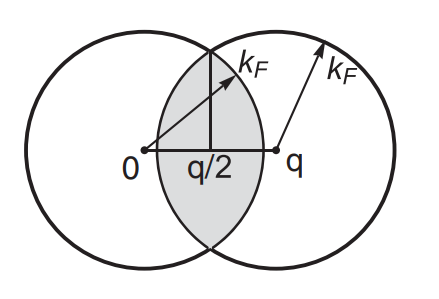
\includegraphics[scale=0.55]{figs/Jellium model/jellium_integration_region.png} }}
    \qquad
    \subfloat[\centering ]{{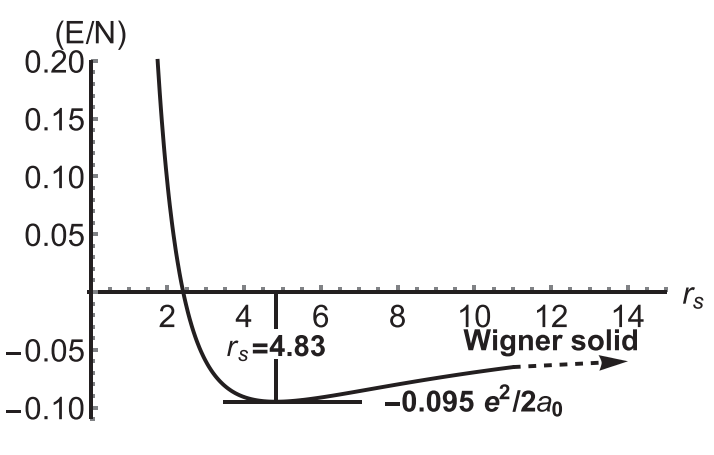
\includegraphics[scale=0.55]{figs/Jellium model/jellium_gse.png}}}
    \caption{Fig. A: Geometry for the ${\bf k}$-integration is shown for arbitrary, but fixed, ${\bf q}$, which is just the intersection of two spheres. \\
    Fig. B: Ground-state energy per electron, including first-order correction, for the jellium model.}
    \label{figs:jellium}
\end{figure}

\begin{equation}
    \begin{split}
        E^{(1)} &= \langle {\Omega} \bigg|  \sum_{\substack{{\bf k},{\bf k}',{\bf q} \in \Lambda\\
    \sigma \in \mathds{C}^2}} \frac{2\pi e^2}{\Omega q^2} {\bf c}_{{\bf k}+{\bf q} \blanky \sigma}^\dagger {\bf c}_{{\bf k}'-{\bf q} \blanky \sigma}^\dagger {\bf c}_{{\bf k}' \blanky \sigma} {\bf c}_{{\bf k} \blanky \sigma} \bigg| {\Omega} \rangle \\
    &= \langle {\Omega} \bigg|  \sum_{\substack{{\bf k},{\bf q} \in \Lambda\\
    \sigma \in \mathds{C}^2}} \frac{2\pi e^2}{\Omega q^2} {\bf c}_{{\bf k}+{\bf q} \blanky \sigma}^\dagger {\bf c}_{{\bf k} \sigma}^\dagger {\bf c}_{{\bf k}+{\bf q} \blanky \sigma} {\bf c}_{{\bf k} \sigma} \bigg| {\Omega} \rangle \\
    &= \langle {\Omega} \bigg|  \sum_{\substack{{\bf k},{\bf q} \in \Lambda\\
    \sigma \in \mathds{C}^2}} \frac{2\pi e^2}{\Omega q^2} (-N_{{\bf k}+{\bf q} \blanky \sigma} - N_{{\bf k} \sigma}) \bigg| {\Omega} \rangle  \Rightarrow \varepsilon^{(1)}({\bf k}) = - \frac{2\pi e^2}{\Omega} \sum_{{\bf q}} \frac{N_{{\bf k}} + {\bf q}}{q^2} \\
    \end{split}
\end{equation}
\begin{equation}
    \begin{split}
    \Rightarrow E^{(1)} &= -\frac{4\pi e^2}{\Omega} \frac{\Omega}{(2\pi)^6} \int_{\mathds{R}^6} d{\bf k} d{\bf q} \blanky \frac{1}{q^2} \Theta(k_F - |{\bf k} + {\bf q}|) \Theta(k_F - k) \textnormal{ with the integration region shown in \cref{figs:jellium} (left)}  \\
    &= - \frac{4\pi e^2 \Omega}{(2\pi)^6} \int_{\mathds{R}^3} \frac{d{\bf q}}{q^2} \int_{\mathds{R}^3} d{\bf p} \blanky \Theta\bigg(k_F - \bigg| {\bf p} + \frac{1}{2} {\bf q}\bigg|\bigg) \Theta\bigg(k_F - \frac{1}{2} {\bf q}\bigg) \\
    &= -\frac{e^2}{2a_0} N \frac{3}{2\pi} \bigg(\frac{9 \pi}{4}\bigg)^{\frac{1}{3}} \frac{1}{r_s}.
    \end{split}
\end{equation}

This results, shown in \cref{figs:jellium} (right), shows that the electron gas is stable when the repulsive Coulomb interaction is turned on. No external confinement potential is therefore needed to hold the electron gas in the ion jellium together. There exists an optimal density $n^*$, or interparticle distance $r_s^*$, which minimizes the energy and furthermore yields an $E^* < 0$. The negative exchange energy overcome the positive kinetic energy. This method of treating the electron gas is a special case of the Hartree-Fock approximation and is the simplest way to take into account interactions. The interesting point to note is that in this approximation the energy is reduced below that of the Sommerfeld gas, which is a manifestation of the exchange hole. 

\begin{figure}
    \centering
    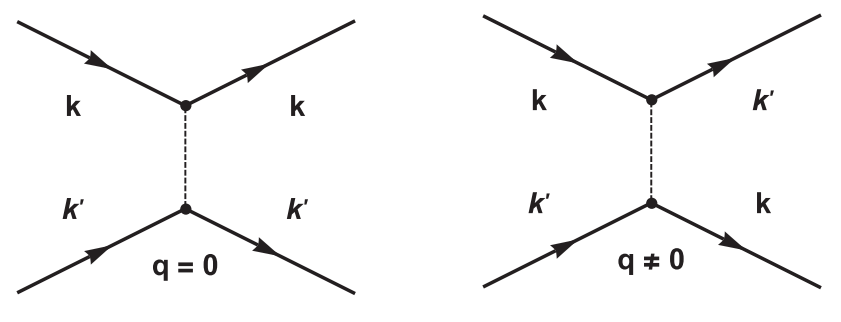
\includegraphics[scale  =.5]{figs/Jellium model/feynmann_diags.png}
    \caption{Diagrams for the jellium sea. The dashed line represents the interaction.}
    \label{fig:feynmann_jellium}
\end{figure}

\blanky \\

\paragraph{\textbf{Hartree-Fock approximation as a Mean-Field Theory}} \label{First_order_Hartree_Fock}\blanky \\

Consider the electronic Hamiltonian given by 
\cref{pre-HF-jellium H}. The goal is to write an effective two-body Hamiltonian, which takes into account the average effects of the interactions. Therefore, the four-Fermi interaction is replaced with a sum of all possible two-body terms

\begin{equation}
    \begin{split}
    \langle {\bf c}_1^\dagger {\bf c}_2^\dagger {\bf c}_3 {\bf c}_4 \rangle_{\textnormal{MFT}} &= - \langle {\bf c}_1^\dagger {\bf c}_3 \rangle {\bf c}_2^\dagger {\bf c}_4 -  \langle {\bf c}_2^\dagger {\bf c}_4 \rangle {\bf c}_1^\dagger {\bf c}_3 +  \langle {\bf c}_1^\dagger {\bf c}_4 \rangle {\bf c}_2^\dagger {\bf c}_3 +  \langle {\bf c}_2^\dagger {\bf c}_3 \rangle {\bf c}_1^\dagger {\bf c}_4, \\
    &\textnormal{ where } \langle {\bf c}_{{\bf k}\sigma}^\dagger {\bf c}_{{\bf k}'\sigma'} \rangle = {\bf n}_{{\bf k}\sigma} \delta_{{\bf k}{\bf k}'}^{\sigma \sigma'}
\end{split}\end{equation}

The mean field terms can be understood as the average number of particles ${\bf n}_{{\bf k}\sigma}$ in the $\ket{{{\bf k}\sigma}}$-state, which will be weighted with the two-body interaction $V({\bf q})$ to give the average interaction due to all other interaction terms. Then, the four-Fermi interaction in the mean-field approximation reads

\begin{equation}
\begin{split}
    \mathcal{V}_{\textnormal{HF}} = \frac{1}{2} \sum_{\substack{{\bf k}{\bf k}',{\bf q} \in \Lambda\\
    \sigma \sigma' \in \mathds{C}^2}} V({\bf q}) &\bigg[-\langle 
    {\bf c}_{{\bf k}\sigma}^\dagger {\bf c}_{{\bf k}'\sigma'}
    \rangle {\bf c}_{{\bf k}'-{\bf q} \blanky \sigma'}^\dagger {\bf c}_{{\bf k}-{\bf q} \sigma} 
    -  \langle {\bf c}_{{\bf k}'-{\bf q} \blanky \sigma'}^\dagger {\bf c}_{{\bf k}-{\bf q} \sigma}  \rangle {\bf c}_{{\bf k}\sigma}^\dagger {\bf c}_{{\bf k}'\sigma'} \\
    & \blanky \blanky \blanky + \langle {\bf c}_{{\bf k}\sigma}^\dagger {\bf c}_{{\bf k}-{\bf q} \sigma} \rangle {\bf c}_{{\bf k}'-{\bf q} \blanky \sigma'}^\dagger {\bf c}_{{\bf k}'\sigma'}
    +  \langle {\bf c}_{{\bf k}'-{\bf q} \blanky \sigma'}^\dagger {\bf c}_{{\bf k}'\sigma'} \rangle {\bf c}_{{\bf k}\sigma}^\dagger {\bf c}_{{\bf k}-{\bf q} \sigma} 
    \bigg] \\
    &= - \sum_{\substack{{\bf k}{\bf q} \in \Lambda\\
    \sigma \in \mathds{C}^2}} V({\bf q})  \langle {\bf c}_{{\bf k} \sigma}^\dagger {\bf c}_{{\bf k} \sigma} \rangle {\bf c}_{{\bf k}-{\bf q} \blanky \sigma}^\dagger {\bf c}_{{\bf k}-{\bf q} \blanky \sigma} + V(0) \sum_{\substack{{\bf k}{\bf k}' \in \Lambda\\
    \sigma \sigma' \in \mathds{C}^2}} \langle {\bf c}_{{\bf k} \sigma}^\dagger {\bf c}_{{\bf k} \sigma} \rangle  {\bf c}_{{\bf k}' \sigma'}^\dagger {\bf c}_{{\bf k}' \sigma'} \\
    &= \sum_{\substack{{\bf k} \in \Lambda\\
    \sigma \in \mathds{C}^2}} \bigg(-\sum_{{\bf q} \in \Lambda} {\bf n}_{{\bf k}+{\bf q} \sigma} V({\bf q}) + nV(0)\bigg){\bf c}_{{\bf k} \sigma}^\dagger {\bf c}_{{\bf k} \sigma}, \\
    \Rightarrow  {\bf H}^{\textnormal{HF}} &= \sum_{\substack{{\bf k} \in \Lambda\\
    \sigma \in \mathds{C}^2}} \varepsilon_{\bf k}^{\textnormal{HF}} {\bf c}_{{\bf k} \sigma}^\dagger {\bf c}_{{\bf k} \sigma}, \textnormal{ where } \begin{split}
        \varepsilon_{\bf k}^{\textnormal{HF}} &= \varepsilon_{\bf k} + \sum_{\substack{{\bf k}' \in \Lambda\\
    \sigma' \in \mathds{C}^2}} [V(0) - \delta_{\sigma\sigma'} V({\bf k}- {\bf k}')] {\bf n}_{{\bf k}' \sigma'} \\
        &= \varepsilon_{\bf k} + V(0) N - \sum_{\substack{{\bf k}' \in \Lambda\\
    \sigma' \in \mathds{C}^2}} V({\bf k}- {\bf k}') {\bf n}_{{\bf k'} \sigma'}.
    \end{split}
    \end{split}
\end{equation}

Note that the Hartree or direct Coulomb term, which represents the average interaction energy of the electron ${\bf k}\sigma$ with all the other electrons in the system, is a constant; when summed over all electron it cancels exactly with the constant arising from the sum of the self-energy of the positive background and the interaction energy of the electron gas with that of the background. The Fock, or exchange term, is a momentum-dependent shift. \\

\textbf{Problems with the Hartree-Fock Theory}

Although we argued that the Hartree-Fock approximation becomes a better approximation in the high-density limit for electron interacting via the Coulomb attraction, it never becomes exact. The Hartree-Fock energy correction is given by 

$$
    \varepsilon^{(1)}({\bf k}) = \frac{e^2 k_F}{4\pi^2} \bigg[\frac{k_F^2 - k^2}{kk_F} \log \bigg| \frac{k_F + k}{k_F - k}\bigg| + 2\bigg]
$$

The first term in parentheses has a logarithmic divergence in slope $k=kf$. This means that while the energy shift might be small compared to the Fermi energy, the Fermi velocity $v_F = \nabla_{{\bf k}} \varepsilon({\bf k})$, contains a non-finite term. This problem can be traced back to the long-range nature of the Coulomb force. Two electrons at large distances ${\bf x}-{\bf x}'$ do not feel the full $\frac{1}{|{\bf x}-{\bf x}'|}$-interaction, but a screened version due to the presence of the intervening medium, namely the electron gas, rearranges itself to cancel out the long-range part of $V$. \\

\underline{Electron Interaction in Second-order Perturbation Theory}

Trying to improve upon the first-order result by going to second-order perturbation theory yields a disastrous results for the matrix elements diverge. According to second-order perturbation theory, 

\begin{equation}
\frac{E^{(2)}}{N} = \frac{1}{N} \sum_{\substack{\ket{\psi} \in \mathds{H} \\
\ket{\psi} \neq \ket{\Omega}}} \frac{\bra{\Omega} {{\bf V}}_c \ket{\psi} \bra{\psi} {{\bf V}}_c \ket{\Omega}}{E^{(0)} - E_\psi}.
\end{equation}

\begin{figure}
    \centering
    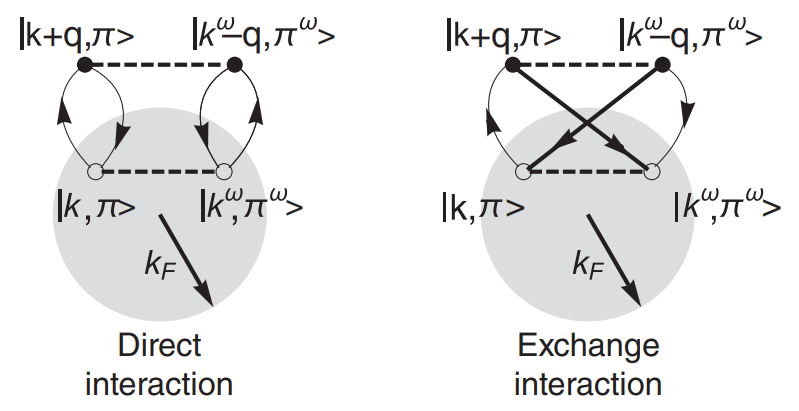
\includegraphics[scale = .5]{figs/Jellium model/fermi_sea_loops_second_order.png}
    \caption{The only two possible processes in second-order perturbation theory for two states, $\ket{{\bf k}_1, \sigma_1}$ and $\ket{{\bf k}_2, \sigma_2}$, in the Fermi sea. The direct process gives a divergent contribution to $\frac{E}{N}$ while the exchange process gives a finite contribution.}
    \label{fig:fermi_sea_loops_second_order}
\end{figure}

This, combined with the momentum-conserving Coulomb interaction, yields intermediate states where two particles are injected out of the Fermi sphere. From such an intermediate state, $\ket{\Omega}$, is restored by putting the excited electrons back into the holes they left behind. Therefore, the are only two types of possible processes: direct interaction and the exchange process, shown in \cref{fig:fermi_sea_loops_second_order}. \\

\begin{enumerate}
    \item In the \underline{Direct interaction}, it turns out that the direct interaction gives a divergent contribution $E^{(2)}_{\textnormal{dir}}$ to $E^{(2)}$ due to the singular behaviour of the Coulomb interaction at small ${\bf q}$-momentum transfers. The $(\ket{\psi} = \ket{\Omega})$-constraint leads to the second p
    
    $$
        \ket{\psi} = \Theta(|{\bf k}_1 + {\bf q}| - k_F) \Theta(|{\bf k}_2 - {\bf q}| - k_F) \Theta(k_F - |{\bf k}_2|) \Theta(k_F - |{\bf k}_1|) {\bf c}_{{\bf k}_1 + {\bf q}}^\dagger {\bf c}_{{\bf k}_2 - {\bf q}}^\dagger {\bf c}_{{\bf k}_2} {\bf c}_{{\bf k}_1} \ket{\Omega}.
    $$
    
    To restore $\ket{\Omega}$,  the same ${\bf q}$-momentum transfer must be involved in both $\bra{\Omega} {\bf V}_c \ket{\psi}$ and $\bra{\psi} {\bf V}_c \ket{\Omega}$, and writing ${\bf V}({\bf q}) = \frac{4 \pi e^2}{{\bf q}^2}$ yields
    
    \begin{equation}
    \begin{split}
    & E^{(2)}_{\textnormal{dir}} = \frac{1}{4 \Omega^2} \sum_{{\bf q} \in \Lambda} \sum_{\substack{{\bf k}{\bf k}' \in \Lambda\\
    \sigma \sigma' \in \mathds{C}^2}} \frac{{\bf V}({\bf q})^2}{E^{(0)} - E_{\nu}} \Theta(|{\bf k}_1 + {\bf q}| - k_F) \Theta(|{\bf k}_2 - {\bf q}| - k_F) \Theta(k_F - |{\bf k}_2|) \Theta(k_F - |{\bf k}_1|) \\
    & \textnormal{Given that ${\bf V}({\bf q})^2 \approx q^{-4}$} \Rightarrow E^{(0)} - E_{\psi} \overset{{\bf q} \rightarrow 0}{\approx} {\bf k}_1^2 + {\bf k}_2^2 - ({\bf k}_1+{\bf q})^2 - ({\bf k}_2 - {\bf q})^2 \approx q \\
    & \sum_{{\bf q} \in \Lambda} \sum_{\substack{{\bf k}{\bf k}' \in \Lambda\\
    \sigma \sigma' \in \mathds{C}^2}} \cdots \Theta(|{\bf k}_2 - {\bf q}| - k_F) \Theta(k_F - |{\bf k}_2|) \Theta(k_F - |{\bf k}_1|)  \overset{{\bf q} \rightarrow 0}{\approx} q \\
    & \Rightarrow E^{(2)}_{\textnormal{dir}} = \int_{0} dq q^2 \frac{1}{q^4} \frac{1}{q} q q = \int_{0} \frac{dq}{q} = \log q|_{0} \rightarrow \infty.
    \end{split}
    \end{equation}
    
    \blanky \\
    
    \item The exchange process does not lead to a divergence since, in this case, the momentum transfer in the excitation part is ${\bf q}$, but in the relaxation part it is ${\bf k}_2-{\bf k}_1-{\bf q}$. Thus ${\bf V}^2({\bf q})$ is replaced by ${\bf V}^2({\bf q}){\bf V}({\bf k}_2-{\bf k}_1-{\bf q}) \propto q^{-2}$ for ${\bf q} \rightarrow 0$, which is less singular than ${\bf V}^2({\bf q}) \propto q^{-4}$. \\  
\end{enumerate}

Physically, the energy of an electron gas must be finite. The only hope for rescue lies in regularization of the divergent behaviour by taking higher-order perturbation terms into account. Consider now the ground-state energy of the jellium model of a three-dimensional electron gas. In the $(r_s < 1)$-regime, this energy can be expressed in terms of a power-series in $r_s$, as

$$
    E_0 = \frac{K}{r_s^2} [1+ br_s + c r_s^2 + \cdots],
$$

where $K, a,b,c$ are constants. This is not exactly right, since first-order perturbation theory gives a term of the $(br_s)$-form in the series. But, considering second-order perturbation theory, one finds a contribution that diverges like $\int_0 \frac{dq}{q}$, where $q$ is the transfer-momentum in the Fourier transform ${\bf V}_q$ of the Coulomb interaction, ${\bf V}_q \approx q^{-2}$. Thus, there is in fact a logarithmic divergence from the lower limit $0$ of the momentum transfers. This divergence is associated with the long range of the Coulomb interaction. Furthermore, if one examines higher-order terms in the perturbation series, one finds that they diverge even more strongly. \\

On physical grounds, however, the energy of the interacting electron gas must be finite and well-defined, with no phase transitions occurring as the repulsive interactions are turned on. This failure of standard perturbation theory appears to signal that the energy does not have a standard power-series expansion in $r_s$. In 1957, Gell-Mann and Bruckner resolved this issue by developing many-body perturbation theory\footnote{Many-body perturbation expansions without diagrams.
I. Normal states. Behnam Farid §}, in which the summation of the divergent terms in the series an infinite number of terms) is performed before doing the momentum integrals, thus arriving to a finite and well-defined results. This is called the resummation of the perturbation series. They found that there was a term in the series for $E_0$ that is $\propto \log r_s$, and is non-analytic at $r_s = 0$. This holds so long the interaction doesn't cause any drastic changes to the system, such as a phase transition. \\

\subsection{Random Phase Approximation}

In the second quantization formalism, the fermionic field operators may be written in plane-wave basis as 

$$
    \Psi({\bf x}, t) = \frac{1}{\sqrt{\Omega}} \sum_{{\bf k} \in \Lambda} e^{i {\bf k} \cdot {\x}} {\bf c}_{{\bf k}}, \blanky \blanky \blanky \blanky 
    \Psi^\dagger({\bf x}, t) = \frac{1}{\sqrt{\Omega}} \sum_{{\bf k} \in \Lambda} e^{-i {\bf k} \cdot {\x}} {\bf c}_{{\bf k}}^\dagger.
$$

The particle density $\rho({\bf x})$ at point ${\bf x}$ is given by 

$$
    \rho({\bf x}) = \sum_{i \in \mathds{N}} \delta({\bf x} - {\bf x}_i) \Rightarrow \rho({\bf x}) = \int_{\mathds{R}^3} d{\bf x} \blanky \Psi^\dagger({\bf x}) \bigg(\sum_{i \in \mathds{N}} \delta({\bf x} - {\bf x}_i)\bigg) \Psi({\bf x}) = \sum_{i \in \mathds{N} }\Psi^\dagger({\bf x}) \Psi({\bf x}). 
$$

Its Fourier transform is given by ${\rho_{{\bf q}}} = \sum_{{\bf k} \in \Lambda} {\bf c}_{{\bf k}+{\bf q}}^\dagger {\bf c}_{\bf k}$. Its physical meaning is straightforward: it gives rise to particle-hole pairs charge fluctuations around the Fermi surface. Since $\rho^\dagger = \rho$, it follows that $\rho_{{\bf q}}^\dagger = \rho_{-{\bf q}}$. \footnote{For example, the following four-body term may be recast as 

$$
\sum_{{\bf k, k'} \in \Lambda} {\bf c}_{{\bf k}-{\bf q}}^\dagger {\bf c}_{{\bf k}'+{\bf q}}^\dagger {\bf c}_{{\bf k}'} {\bf c}_{{\bf k}} = - \sum_{{\bf k'} \in \Lambda} {\bf n}_{{\bf k}'} + \rho_{{\bf q}} \rho_{-{\bf q}'}.
$$}\\

Now, the following question naturally arises. Under what conditions an interacting system, with Hamiltonian 

$$
    {\bf H} = \sum_{{\bf k} \in \Lambda} \varepsilon_{{\bf k}} {\bf c}_{{\bf k}}^\dagger {\bf c}_{{\bf k}} + \frac{1}{2} \sum_{{\bf q} \in \Lambda} {\bf V}_{{\bf q}} (\rho_{{\bf q}} \rho_{-{\bf q}} - N),
$$

and ground-state $\ket{\Omega}$, ${\bf H} \ket{\Omega} = \varepsilon_0 \ket{\Omega}$, can support density excitations associated with $\rho_{{\bf q}}$? Namely, these excitations are

$$
    {\bf H} \rho_{{\bf q}}^\dagger \ket{\Omega} = (\varepsilon_0 + \hbar \omega_{{\bf q}}) \rho_{{\bf q}}^\dagger \ket{\Omega}
$$

\blanky \\

The previous equation may be rewritten as 

\begin{equation} 
\begin{split}
    [{\bf H}, \rho_{\bf q}^\dagger] = \hbar \omega_{{\bf q}} \rho_{{\bf q}}^\dagger  \Rightarrow & \bigg[\sum_{{\bf k} \in \Lambda} \varepsilon_{{\bf k}} {\bf c}_{{\bf k}}^\dagger {\bf c}_{{\bf k}} + \frac{1}{2} \sum_{{\bf q} \in \Lambda} {\bf V}_{{\bf q}} (\rho_{{\bf q}} \rho_{-{\bf q}} - N), \rho_{\bf q}^\dagger \bigg] = \hbar \omega_{{\bf q}} \rho_{{\bf q}}^\dagger \\
    & \bigg[\sum_{{\bf k} \in \Lambda} \varepsilon_{{\bf k}} {\bf c}_{{\bf k}}^\dagger {\bf c}_{{\bf k}}, \rho_{\bf q}^\dagger\bigg] + \frac{1}{2} \bigg[\sum_{{\bf q} \in \Lambda} {\bf V}_{{\bf q}} (\rho_{{\bf q}} \rho_{-{\bf q}} - N), \rho_{\bf q}^\dagger \bigg] = \\
    & \sum_{{\bf k} \in \Lambda} \varepsilon_{{\bf k}} \bigg[ {\bf c}_{{\bf k}}^\dagger {\bf c}_{{\bf k}}, \rho_{\bf q}^\dagger\bigg] + \frac{1}{2} \sum_{{\bf q} \in \Lambda} {\bf V}_{{\bf q}} \cancel{\bigg[\rho_{{\bf q}} \rho_{-{\bf q}}, \rho_{\bf q}^\dagger\bigg]} = \\
    & \sum_{{\bf k}, \mathfrak{k} \in \Lambda} \varepsilon_{{\bf k}} \bigg[ {\bf c}_{{\bf k}}^\dagger {\bf c}_{{\bf k}}, {\bf c}_{{\bf q}} {\bf c}_{{\bf \mathfrak{k} + q}}^\dagger \bigg] =  \\
    &\sum_{{\bf k}, \mathfrak{k} \in \Lambda} \varepsilon_{{\bf k}} \bigg({\bf c}_{{\bf k}}^\dagger \cancel{[{\bf c}_{{\bf k}}, {\bf c}_{{\bf q}}]} {\bf c}_{{\bf \mathfrak{k} + q}}^\dagger + [{\bf c}_{{\bf k}}^\dagger, {\bf c}_{{\bf q}}] {\bf c}_{{\bf k}} {\bf c}_{{\bf k}}^\dagger + {\bf c}_{{\bf q}} {\bf c}_{{\bf k}}^\dagger [{\bf c}_{{\bf k}}, {\bf c}_{{\bf \mathfrak{k} + q}}^\dagger] + {\bf c}_{{\bf q}} \cancel{[{\bf c}_{{\bf k}}^\dagger, {\bf c}_{{\bf \mathfrak{k} + q}}^\dagger]} {\bf c}_{{\bf k}} \bigg) = \\
    & \sum_{{\bf k} \in \Lambda} (\varepsilon_{{\bf k + q}} - \varepsilon_{{\bf k}}) {\bf c}_{{\bf {\bf k} + q}}^\dagger {\bf c}_{{\bf k}} = 
\end{split}
\end{equation}

If $\rho_{{\bf q}}^\dagger$ actually creates an excitation of energy $\hbar \omega$, then 

\begin{equation}
\begin{split}
    [{\bf H}, [{\bf H}, \rho_{\bf q}^\dagger]] = (\hbar \omega)^2 \rho_{{\bf q}}^\dagger \\
    \Rightarrow (\hbar \omega)^2 \rho_{{\bf q}}^\dagger &= \sum_{{\bf k} \in \Lambda} (\varepsilon_{{\bf k + q}} - \varepsilon_{{\bf k}}) [{\bf H}, {\bf c}_{{\bf {\bf k} + q}}^\dagger {\bf c}_{{\bf k}}] = \sum_{{\bf k} \in \Lambda} (\varepsilon_{{\bf k + q}} - \varepsilon_{{\bf k}})^2 {\bf c}_{{\bf k + q}}^\dagger {\bf c}_{{\bf k}} \\
    & \blanky \blanky \blanky \blanky+ \sum_{{\bf k}, {\bf q}' \in \Lambda} (\varepsilon_{{\bf k + q}} - \varepsilon_{{\bf k}}) \frac{V_{{\bf q}'}}{2} \bigg[({\bf c}_{{\bf {\bf k} + q - q'}}^\dagger {\bf c}_{{\bf k}} - {\bf c}_{{\bf k + q}}^\dagger {\bf c}_{{\bf {\bf k} + q'}}) \rho_{{\bf q}'}^\dagger + \rho_{{\bf q}'} ({\bf c}_{{\bf {\bf k} + q + q'}}^\dagger {\bf c}_{{\bf k}} - {\bf c}_{{\bf k + q}}^\dagger {\bf c}_{{\bf {\bf k} - q'}})\bigg] \\
    &= \sum_{{\bf k} \in \Lambda} \bigg[ \frac{\hbar^2}{2m} (2 {\bf k} \cdot {\bf q} + {\bf q}^2)\bigg]^2 {\bf c}_{{\bf k}+{\bf q}}^\dagger {\bf c}_{{\bf k}} + \sum_{{\bf k}, {\bf q}' \in \Lambda} \frac{V_{\bf q'}}{2}\bigg[\frac{\hbar^2}{2m}(2 {\bf k}\cdot {\bf q} + {\bf q}^2) ({\bf c}_{{\bf {\bf k} + q - q'}}^\dagger {\bf c}_{{\bf k}} - {\bf c}_{{\bf k + q}}^\dagger {\bf c}_{{\bf {\bf k} + q'}}) \\ & \blanky \blanky \blanky \blanky - \frac{\hbar^2}{2m}(2 {\bf k}\cdot {\bf q} + {\bf q}^2) ({\bf c}_{{\bf {\bf k} + q + q'}}^\dagger {\bf c}_{{\bf k}} - {\bf c}_{{\bf k + q}}^\dagger {\bf c}_{{\bf {\bf k} - q'}})\bigg] \\
    &= \sum_{{\bf k} \in \Lambda} \bigg[ \frac{\hbar^2}{2m} (2 {\bf k} \cdot {\bf q} + {\bf q}^2)\bigg]^2 {\bf c}_{{\bf k}+{\bf q}}^\dagger {\bf c}_{{\bf k}} + \sum_{{\bf q}' \in \Lambda} \frac{V_{\bf q'}}{2} \bigg[ \sum_{{\bf k} \in \Lambda}\frac{\hbar^2}{2m}(2 {\bf k}\cdot {\bf q} + {\bf q}^2) ({\bf c}_{{\bf {\bf k} + q - q'}}^\dagger {\bf c}_{{\bf k}} - {\bf c}_{{\bf k + q}}^\dagger {\bf c}_{{\bf {\bf k} + q'}}) \\ 
    & \blanky \blanky \blanky \blanky - \sum_{{\bf k} \in \Lambda}\frac{\hbar^2}{2m}(2 {\bf k}\cdot {\bf q} + {\bf q}^2) ({\bf c}_{{\bf {\bf k} + q + q'}}^\dagger {\bf c}_{{\bf k}} - {\bf c}_{{\bf k + q}}^\dagger {\bf c}_{{\bf {\bf k} -
    q'}})\bigg] \\
    &= \sum_{{\bf k} \in \Lambda} \bigg[ \frac{\hbar^2}{2m} (2 {\bf k} \cdot {\bf q} + {\bf q}^2)\bigg]^2 {\bf c}_{{\bf k}+{\bf q}}^\dagger {\bf c}_{{\bf k}} \\
    & + \sum_{{\bf q}' \in \Lambda} \frac{V_{\bf q'}}{2} \bigg[ \sum_{{\bf k} \in \Lambda}\frac{\hbar^2}{2m}(2 {\bf k}\cdot {\bf q} + {\bf q}^2) {\bf c}_{{\bf {\bf k} + q - q'}}^\dagger {\bf c}_{{\bf k}} - \frac{\hbar^2}{2m}(2 {\bf k}\cdot {\bf q} + {\bf q}^2) {\bf c}_{{\bf k + q}}^\dagger {\bf c}_{{\bf {\bf k} + q'}} \\
    & \blanky \blanky \blanky \blanky - \sum_{{\bf k} \in \Lambda}\frac{\hbar^2}{2m}(2 {\bf k}\cdot {\bf q} + {\bf q}^2) {\bf c}_{{\bf {\bf k} + q + q'}}^\dagger {\bf c}_{{\bf k}} - \frac{\hbar^2}{2m}(2 {\bf k}\cdot {\bf q} + {\bf q}^2) {\bf c}_{{\bf k + q}}^\dagger {\bf c}_{{\bf {\bf k} - q'}}\bigg] \\
    \end{split}
\end{equation}

\begin{equation}
    \begin{split}
 \blanky  
&= \sum_{{\bf k} \in \Lambda} \bigg[ \frac{\hbar^2}{2m} (2 {\bf k} \cdot {\bf q} + {\bf q}^2)\bigg]^2 {\bf c}_{{\bf k}+{\bf q}}^\dagger {\bf c}_{{\bf k}} \blanky \blanky \blanky \blanky \blanky \blanky \textnormal{  let ${\bf k}' = {\bf k} + {\bf q}'$, ${\bf k}'' = {\bf k} - {\bf q}'$}\\
 & \blanky \blanky \blanky \blanky + \sum_{{\bf q}' \in \Lambda} \frac{V_{\bf q'}}{2} \bigg[ \sum_{{\bf k} \in \Lambda}\frac{\hbar^2}{2m}(2 {\bf k}\cdot {\bf q} + {\bf q}^2) {\bf c}_{{\bf {\bf k} + q - q'}}^\dagger {\bf c}_{{\bf k}} - \sum_{{\bf k}' \in \Lambda}\frac{\hbar^2}{2m}(2 ({\bf k}' - {\bf q}')\cdot {\bf q} + {\bf q}^2) {\bf c}_{{\bf k' + q - q'}}^\dagger {\bf c}_{{\bf {\bf k}'}}\\ 
 & \blanky \blanky \blanky \blanky - \sum_{{\bf k} \in \Lambda}\frac{\hbar^2}{2m}(2 {\bf k}\cdot {\bf q} + {\bf q}^2) {\bf c}_{{\bf {\bf k} + q + q'}}^\dagger {\bf c}_{{\bf k}} - \sum_{{\bf k}'' \in \Lambda}\frac{\hbar^2}{2m}(2 ({\bf k}'' + {\bf q}')\cdot {\bf q} + {\bf q}^2) {\bf c}_{{\bf k'' + q + q'}}^\dagger {\bf c}_{{\bf {\bf k}''}} \bigg] \\
    \end{split}
\end{equation}

\begin{align}
     \alignedbox{(\hbar \omega)^2 \rho_{{\bf q}}^\dagger}{= \sum_{{\bf k} \in \Lambda} \bigg[ \frac{\hbar^2}{2m} (2 {\bf k} \cdot {\bf q} + {\bf q}^2)\bigg]^2 {\bf c}_{{\bf k}+{\bf q}}^\dagger {\bf c}_{{\bf k}} + \sum_{{\bf q}' \in \Lambda} \frac{V_{\bf q'}}{2} \frac{\hbar^2 {\bf q} \cdot {\bf q}'}{m} \bigg(\rho_{{\bf q}' - {\bf q}} \rho_{{\bf q}'}^\dagger - \rho_{{-{\bf q}'}}^\dagger \rho_{-{\bf q} - {\bf q}'} \bigg).}
     \label{RPA-basis equation}
\end{align}

\begin{figure}
    \centering
    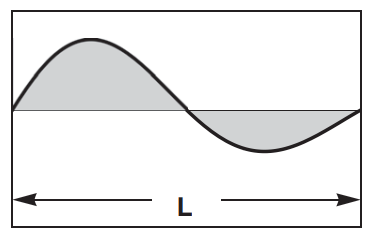
\includegraphics[scale = .5]{figs/Jellium model/RPA-fig.png} 
    \caption{Consider a length-$L$ box. Then, $\rho_q$ measures the quantity approximately equal to the difference in the particle number in the two halves of the container. }
    \label{fig:RPA-box}
\end{figure}

Now, in order to study \cref{RPA-basis equation}, note that $\rho_0$ is actually much larger than all the other components. It is just the average particle density in the system. Consider a box of length-$L$, shown in \cref{fig:RPA-box}, containing a large number of electrons of $\rho_0$ average density, then $\rho_0$'s first Fourier component is 

$$
    \int_{\Omega \subset \R^3} d{\bf x} \blanky \rho({\bf x}) e^{\frac{2i \pi x}{L}},
$$

will be approximately equal to the difference between the particle number in the left and right hand sides of the box, the gray area. The number difference will then be small, compared to the total number and so $\rho_0$ will prevail in the summation over ${\bf q}'$. Since the $({\bf q}' = 0)$-term is omitted, $\rho_0$ will only appear when ${\bf q}' = \pm {\bf q}$. The neglect of all other terms, when ${\bf q}' \neq \pm {\bf q}$ is known as the \textbf{random phase approximation} \footnote{An alternative interpretation for the RPA is as follows. Consider the first-quantized version of the density operator $\rho_{{\bf q} \in \Lambda} = \frac{1}{\Omega} \sum_{n \in \mathds{N}} e^{i {\bf q} \cdot {\bf x}_n}$, where ${\bf x}_n$ is the $n$-th's particles position. Then, $\rho_{{\bf q} \pm {\bf q}'}$ may be written in first quantized form as 

$$
    \rho_{{\bf q} \pm {\bf q}'} \frac{1}{\Omega} \sum_{n \in \mathds{N}} e^{i ({\bf q} \pm {\bf q}') \cdot {\bf x}_n}.
$$

Then, if the electrons are statistically randomly distributed in the system, the preceding sum only gives a finite result if ${\bf q} = \mp {\bf q'}$, since the sum involves random phases that add destructively. In RPA, \cref{RPA-basis equation} is approximated by keeping only terms with ${\bf q} = \mp {\bf q}'$. }.\\

\underline{Plasma oscillations}

Consider the case where ${\bf q}$ is small enough that, for the moment, the first term in \cref{RPA-basis equation} may be neglected and the second term approximated via RPA. In that case, 

$$
(\hbar \omega)^2 \rho_{{\bf q}}^\dagger = \frac{4\pi e^2}{q^2} \frac{\hbar^2 q^2}{m} (\rho_0 \rho_{{\bf q}}^\dagger + \rho_{{\bf q}}^\dagger \rho_0 ) \rightarrow \omega^2 = \frac{4\pi e^2 \rho_0}{m},
$$

which gives just the classical plasma frequency $\omega_P$. The contribution of the first term may be approximated by setting $k \sim k_F$ and $\langle 2 {\bf k}_F \cdot {\bf q} \rangle >> {\bf q}^2$. Averaging over all angles yields

$$
\langre ({\bf k}_F \cdot {\bf q})^2 \rangle \simeq \frac{1}{4\pi} 4\pi^2 k_F^2 q^2 \int_{-1}^{1} dx x^2 = 2\pi k_F^2 q^2, 
$$

which yield the plasmon dispersion relation

$$
\omega^2({\bf q}) = \omega_P^2 + \frac{2\pi \hbar^2 k_F^2}{3m^2} q^2 \simeq \omega_P + \frac{\pi v_F^2}{3\omega_P} q^2. 
$$

Thus, the relevant long-wavelength excitations are collective motions of the electron gas. Bohm and Pines suggested that electrons act as interacting particles through a bare Coulomb potential $\frac{4\pi e^2}{q^2}$ only for length scales less than an effective screening length, which may be taken to be the Thomas-Fermi distance, $\sim q_{\textnormal{TF}}^{-1}$. Below $q_{\textnormal{TF}}$, the interaction contribute only to the plasma oscillations. \\

\paragraph{.}
